% \documentclass[a4paper,12pt,twoside]{report}
\documentclass{llncs}
\usepackage[left=2cm,right=2cm,top=2cm,bottom=3cm]{geometry}
\usepackage[utf8]{inputenc}
\usepackage{graphicx}
% \usepackage{caption}
\usepackage{multirow}
\usepackage{algorithm}% http://ctan.org/pkg/algorithms
\usepackage{algpseudocode}% http://ctan.org/pkg/algorithmicx
% \usepackage{subcaption}
% \usepackage{epigraph}
\usepackage{amsmath}
\usepackage{fixltx2e}
% \usepackage{amssymb}
% \usepackage{mathptmx}
\usepackage{tikz}
\usetikzlibrary{arrows,shapes,positioning,mindmap,trees,automata}
\providecommand{\keywords}[1]{\textbf{\textit{Mots-clés --}} #1}

\newcommand{\textoverline}[1]{$\overline{\mbox{#1}}$}
\newcommand*\circled[1]{\tikz[baseline=(char.base)]{
            \node[shape=circle,draw,inner sep=2pt] (char) {#1};}}
\begin{document}

\title{From motion effects to affordances: Bayesian learning of high-level actions}

\author{Stanislas Leroy\\
   Master 2 parcours Intelligence Artificielle\\
   2016-2017\\
   Département Informatique\\
   Encadrants : Stéphane Doncieux et Alexandre Coninx}

\institute{Institut des Systèmes Intelligents et de Robotique\\
Université Claude Bernard Lyon 1, France}
  % Put your university logo here if you wish.
  %  \begin{center}
  %  
\includegraphics[width=0.5\textwidth]{figures/logo-lyon1.png}
  %  \end{center}
\maketitle

\keywords{Robotique développementale, affordance, clusterisation d'effets}

% \tableofcontents





\section*{Remerciements}
% \addcontentsline{toc}{chapter}{Acknowledgement}

Mon stage de 6 mois au sein de l'équipe AMAC à l'ISIR fût une formidable expérience. Je voudrai remercier Stéphane Doncieux, Alexandre Coninx et Carlos Maestre pour leur support et les nombreux conseils avisés qu'ils m'ont donnés. En effet, bénéficier de leur expérience et savoirs a été un véritable atout pour mener à bien ce stage, notamment pour surmonter les nombreux défis auxquels j'ai été confrontés.

L'ISIR est un excellent laboratoires de robotique en France et avoir la possibilité d'y faire un stage a été une extraordinaire opportunité, notamment parce que j'ai pu travailler sur un domaine passionnant et relativement jeune : la robotique développementale. Par ailleurs, cette immersion dans un laboratoire de recherche m'a donné l'opportunité de découvrir davantage le monde de la recherche.

D'autre part, reprendre des études en septembre 2016 après avoir travaillé plusieurs années a été un véritable défi pour moi. En effet, cela supposait de quitter la ville où je vivais, mes amis et mon confort matériel ainsi que de revenir sur les bancs de l'université. J'allais avoir 30 ans et je me demandais si j'allais réussir dans ce Master 2.

% I am very glad to have the opportunity to pursue my works in PhD in the current months.



% \epigraph{If I have seen further, it is by standing on the shoulders of giants.}{\textit{Isaac Newton}}
\section{Introduction}

Présentation du laboratoire dans lqauel j'ai réalisé mon stage, puis ensuite le projet, mon travail théorique puis une expérimentation basée sur celui-ci. Enfin, discussion et conclusion

\section{Le laboratoire}

L'ISIR\footnote{http://www.isir.upmc.fr} (Institut des Systèmes Intelligents et de Robotique) est un laboratoire de recherche multi-disciplinaire créé en 2007. C'est une Unité Mixte de Recherche entre UPMC et le CNRS, localisé sur le campus de Jussieu. Il compte environ 130 personnes et rassemble des chercheurs de différents domaines : Sciences de l’Ingénieur et de l’Information ainsi que des Sciences du Vivant. Par ailleurs, l'ISIR est membre du réseau national Robotex\footnote{http://equipex-robotex.fr} qui regroupe des plates-formes expérimentales de robotique en France.

Les travaux de recherche à l'ISIR sont principalement centrés sur la modélisation et l'analyse des systèmes dynamiques artificiels et naturels, la conception optimale de systèmes robotiques interactifs, la commande des systèmes interactifs, la conception et le traitement du signal de systèmes perceptifs multimodaux, la modélisation des interactions homme - système, les modèles neuro-computationnels pour l’autonomie, l'apprentissage artificielle, l'adaptation bio-inspirée des systèmes et de leur commande. Dans cette perspective, le laboratoire est consitué de 4 équipes :
\begin{itemize}
\item AGATHE (Assistance aux Gestes et Applications THErapeutiques) : conception de systèmes robotiques synergétiques pour en particulier le guidage des gestes dans des applications thérapeutiques
\item AMAC (Architectures et Modèles pour l'Adaptation et la Cognition) : apprentissage artificiel et l’adaptation du comportement à l’environnement
\item INTERACTION : processus d’interaction avec des mondes physiques et virtuels ou les agents en interaction peuvent être des personnes, des machines, des robots, des avatars virtuels ou des dispositifs physiques
\item SYROCCO (SYstèmes RObotiques COmplexes) : commande des systèmes robotiques dynamiques adaptatifs et leur conception par notamment des méthodes d’optimisation et de synthèse de fonctions bio-inspirées
\end{itemize}

J'ai réalisé mon stage de fin d'études au sein de l'équipe AMAC, dirigée par Stéphane Doncieux. L'équipe est composée de 13 membres permanents et 6 membres non-permanents. Plusieurs membres sont spécialisés en neurosciences tandis que d'autres sont experts en robotique.


Nombre de personnes
Date de création, co-tutelle
Groupe de travail

http://www.isir.upmc.fr/telechargements/Rapport_activite_18_10_2012.pdf

AMAC : thématique de recherche


\section{Le projet DREAM}
Mon stage a été financé dans le cadre le projet DREAM\footnote{http://www.robotsthatdream.eu}. DREAM (Deferred Restructuring of Experience in Autonomous Machines) soit Restructuration différée de l'expérience dans les machines autonomes est un projet financé par le programme de recherche et d'innovation H2020 de l'Union Européenne. Ce projet a pour objectif d'incorporer un processus de sommeil et l'équivalent de rêves au sein d'une architecture cognitive, dans le but de consolider leur expérience et donc améliorer leur capacité à apprendre et à s'adapter.

Une partie des membres de l'équipe AMAC travaille sur le projet DREAM (3 chercheurs, 2 post-doctorants, 3 doctorants et 4 stagiaires).
Seung Su, Léni et Jonathan : tracking d'objets et création de \textit{saliency map}.

Par exemple, plusieurs personnes travaillent sur la perception interactive. L'idée principale de la discipline est que pour segmenter des éléments (en l'occurrence des objects manipulables) dans une scène quelconque on ne peut pas se baser sur un a priori. Pour compenser cela, l'on va interagir avec l'environnement afin d'acquérir cette information. Le but d'un babillage est donc de produire une base de données. Une partie consiste à segmenter ce qui bouge et une autre doit pouvoir segmenter chaque objet. La segmentation de Leni me permet d'initialiser des hypothèses d'objets (ensemble de supervoxels) avec lesquels le robot interagit afin de valider ou non l'appartenance des supervoxels à un unique objet. La base de données qui est construite contient pour chaque objet les exemples de supervoxels qui lui ont été attribué.

Carlos : Apprentissage d'affordance
Pierre : reconnaissance de formes ?

Les différents partenaires académiques disposent de 5 robots pour mener à bien ce projet : le robot Meka\footnote{http://en.wikipedia.org/wiki/Meka\_Robotics}, PR2 de Willow Garage, plusieurs Thymio-2\footnote{www.thymio.org/}, le bras robotique CrustCrawler\footnote{http://www.crustcrawler.com} ainsi que le robot Baxter de Rethink Robotics. La majorité des robots est présente au sein de l'ISIR.

Conditions controlées où tout est connu à l'avance (possible de programmer explicitement le robot à résoudre une tâche) à des environments ouverts où les concepts peuvent changer au cours du temps et où de nouveaux concepts peuvent apparaître. Il faut donc programmer le robot pour qu'il soit autonome et adaptable.

Motivation du projet : Concevoir un système développemental capable de démarrer depuis une représentation agnostique et switcher, de façon progressive et autonome, vers des représentations plus adaptées. Question : comment boostraper ?

Where to start from?
- Task agnostic system, no specific representation imposed
- Raw sensorimotor flow
- Basic motivation system
What mechanisms for the system to develop?
- cognitive architecture relying on evolutionary algorithms
- What information is relevant?
- Information found to be relevant to satisfy motivations while exploring
possible behaviors
How to store it and use it to make the robot more efficient the day after?
- By constructing models and \textit{redescribing} their representation to make
them more compact and more accurate during robot’s \textit{dreams}

evolutionary approach to
development : alternating between
• active interaction (daytime) and
• passive introspection over past
events (nighttime and dreams)

Le projet DREAM comprend 4 objectifs : (1) Faire évoluer et décompoer de nouvelles valeurs et motivations, (2) Restructurer les représentations et modèles, (3) Consolider la connaissance et (4) expand la connaissance à travers les interactions sociales.

\begin{figure}
	\centering
	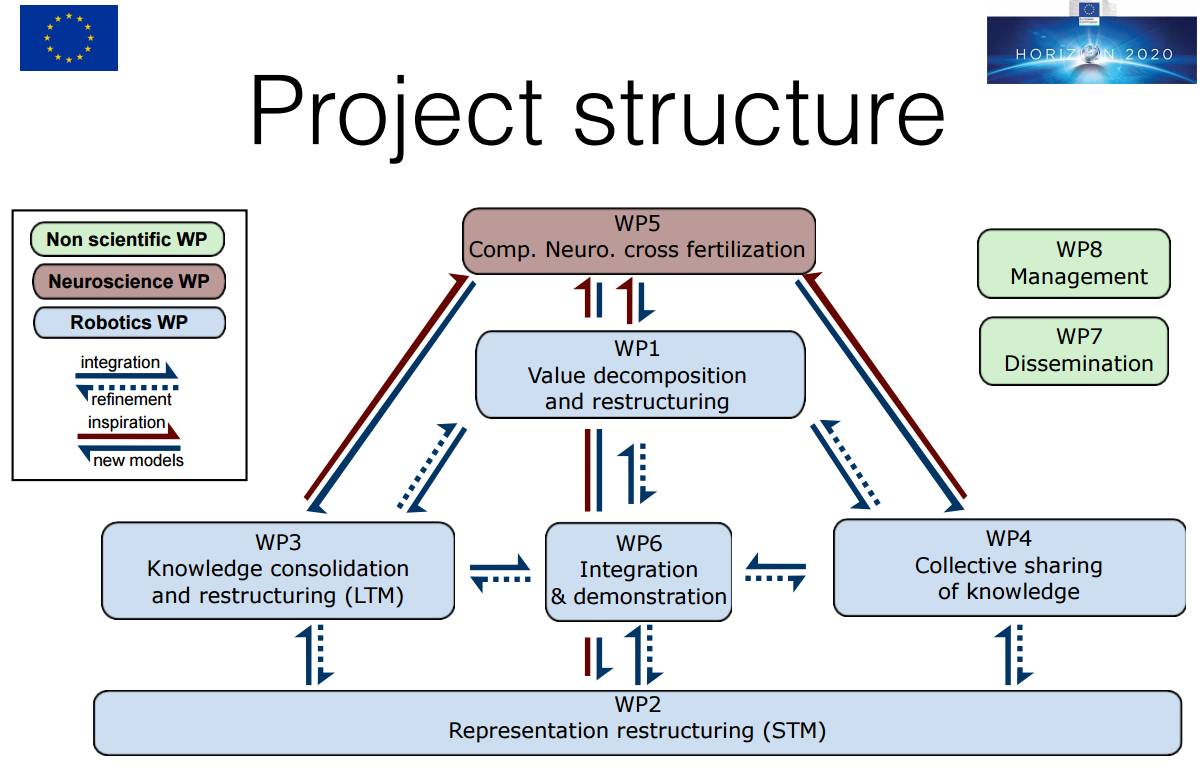
\includegraphics[width=.7\textwidth]{figures/project_structure.png}
	\label{fig:dream}
	\caption{Baxter robot}
\end{figure}

Accumuler de la connaissance nécessite des processus de consolidation afin d'éviter d'être submergé par les informations. Le sommeil crucial pour la restructuration des représentations, maintenir l'intégratione et la cohérence de la connaissance, amélioration de l'apprentissage et la formation d'abstraction.

Permettre aux robots d'acquérir une représentation ouverte du monde. Alterner périodes d'expériences et de sommeil.

Jusqu'à présent, le rôle du sommeil a été négligé dans l'IA et la robotique.

Selon DREAM, le cerveau de compose de 3 sous-systèmes : modèles, politique, valeurs.

Alternance entre interaction active et introspection passive.

Détails du projet Dream.
Détails des différents objectifs.
Description des différentes waves.
Le projet DREAM est scindé en 13 étapes, appelées \textit{waves} dont la liste est donnée en annexe réparties au sein de 8 Work Packages \ref{fig:dream}.

Au terme de ce projet, les différents travaux de recherche des différents membres ont vocation à s'imbriquer les uns avec les autres dans le but de fournir un système global, allant de la détection et le suivi d'objet, à l'apprentissage d'affordances en passant par l'apprentissage de lancers de balle.

La Coruna : travaux sur les motivations extrinsèques.

Plusieurs expériences sont prévues afin de valider les travaux effectués. La première consiste en un robot avec un bras. Le robot doit placer différents objets dans une zone particulière ou presser des boutons et manipuler des leviers. La deuxième expérience de validation consiste à collecter des balles.

Finalement, pluisieurs résultats sont attendus à l'issue de ce projet. Domaine de la robotique : de nouveaux frameworks pour le boostrapping cognitif, qui s'appuie sur des algorithmes évolutionnaires, avec une alternance entre des phases actives et passives (jour/nuit) et avec des connaissances approfondies en psychologie et neurosciences. Du point de vue des neurosciences, de nouveaux modèles pour la restructuration de connaissance et le bootstrapping cognitif.





\subsection{\'Etat de l'art}

% Medias are nowadays talking about smart robots for tomorrow or the day after tomorrow. Such mass medias are explaining that people would find in their house, in a very near future,  a robot able to cook for you when you are short in time, mow the lawn and take care of elder people. However the path which conducts to these intelligent machines is still long and strewn with pitfalls. Several challenges have to be adressed before people interact with those robots as they do with other human people. Among these challenges, it is possible to cite movements learning.

% Developmental robotics
\subsubsection{Robotique développementale}
La robotique moderne est apparue au début du siècle dernier et englobe la robotique industrielle, médicale, militaire et domestique. Si l'on s'y rapporte, la robotique développementale constitue un domaine de recherche relativement jeune dans la mesure où son émergence date d'une quinzaine d'années. La robotique développementale est issue principalement de la robotique mais tire également ses racines des neurosciences cognitives.
Apprentissage autonome, généralisation.
Plus efficace de créer un robot qui apprend qu'un robot auquel on apprend beaucoup de choses.
Cf. wikipedia




%% Affordances
% Affordances are an important concept when talking about sensorimotor learning. The term was defined in \cite{opac-b1085639} as what \textit{it offers the animal, what it provides or furnishes}. The main idea behing that term is to be able to discover the different actions that can be performed on an object, by considering available abilities. That definition establishes a strong relation between objects, actions and effects (see Figure \ref{fig:affordances}). For instance, for a robot with a grasper, affordances on a simple box are: pushing, grasping or touching. Furthermore, affordances can be also used to identify or reproduce action as described in \cite{4399517}.
% Affordances are objective, real and physical.
\subsubsection{Affordances}
L'apprentissage des affordances est une étape cruciale dans l'approche de la robotique développementale. Le terme a été défini dans \cite{opac-b1085639} comme \textit{it offers the animal, what it provides or furnishes}. L'idée principale derrière ce terme est d'être capable de découvrir les différentes actions qui peuvent être réalisées sur un objet, en considérant les capacités disponibles. Cette définition établit une relation forte entre les objets, les actions et les effets (see Figure \ref{fig:affordances}). Les affordances permettent de découvrir les différentes actions qui peuvent être réalisées sur un objet en fonction des capacités de l'acteur. Par exemple, pour un robot avec des pinces, une boîte offre les affordances  \textit{movable} et \textit{levable}, parmi d'autres. Les affordances sont capitables pour réaliser des actions, c'est-à-dire que le robot peut utiliser sa connaissance des affordances pour choisir la prochaine action à effectuer sur un objet pour accomplir une tâche. Par ailleurs, les affordances peuvent également être utilisées pour identifier ou reproduire des actions, telles qu'expliqué dans \cite{4399517}.

 %
 % A babbling approach consisting in applying random action and observing the corresponding effects can provide the data required to learn it, but where to start from? Defining a priori a limited set of possible actions and corresponding effects is a strong limitation to what the robot can achieve, but applying completely random actions results in a large set of possible effects that may be hard to exploit, in particular if the affordance is represented with a Bayesian network \cite{}.

% \begin{figure}
% 	\centering
% 	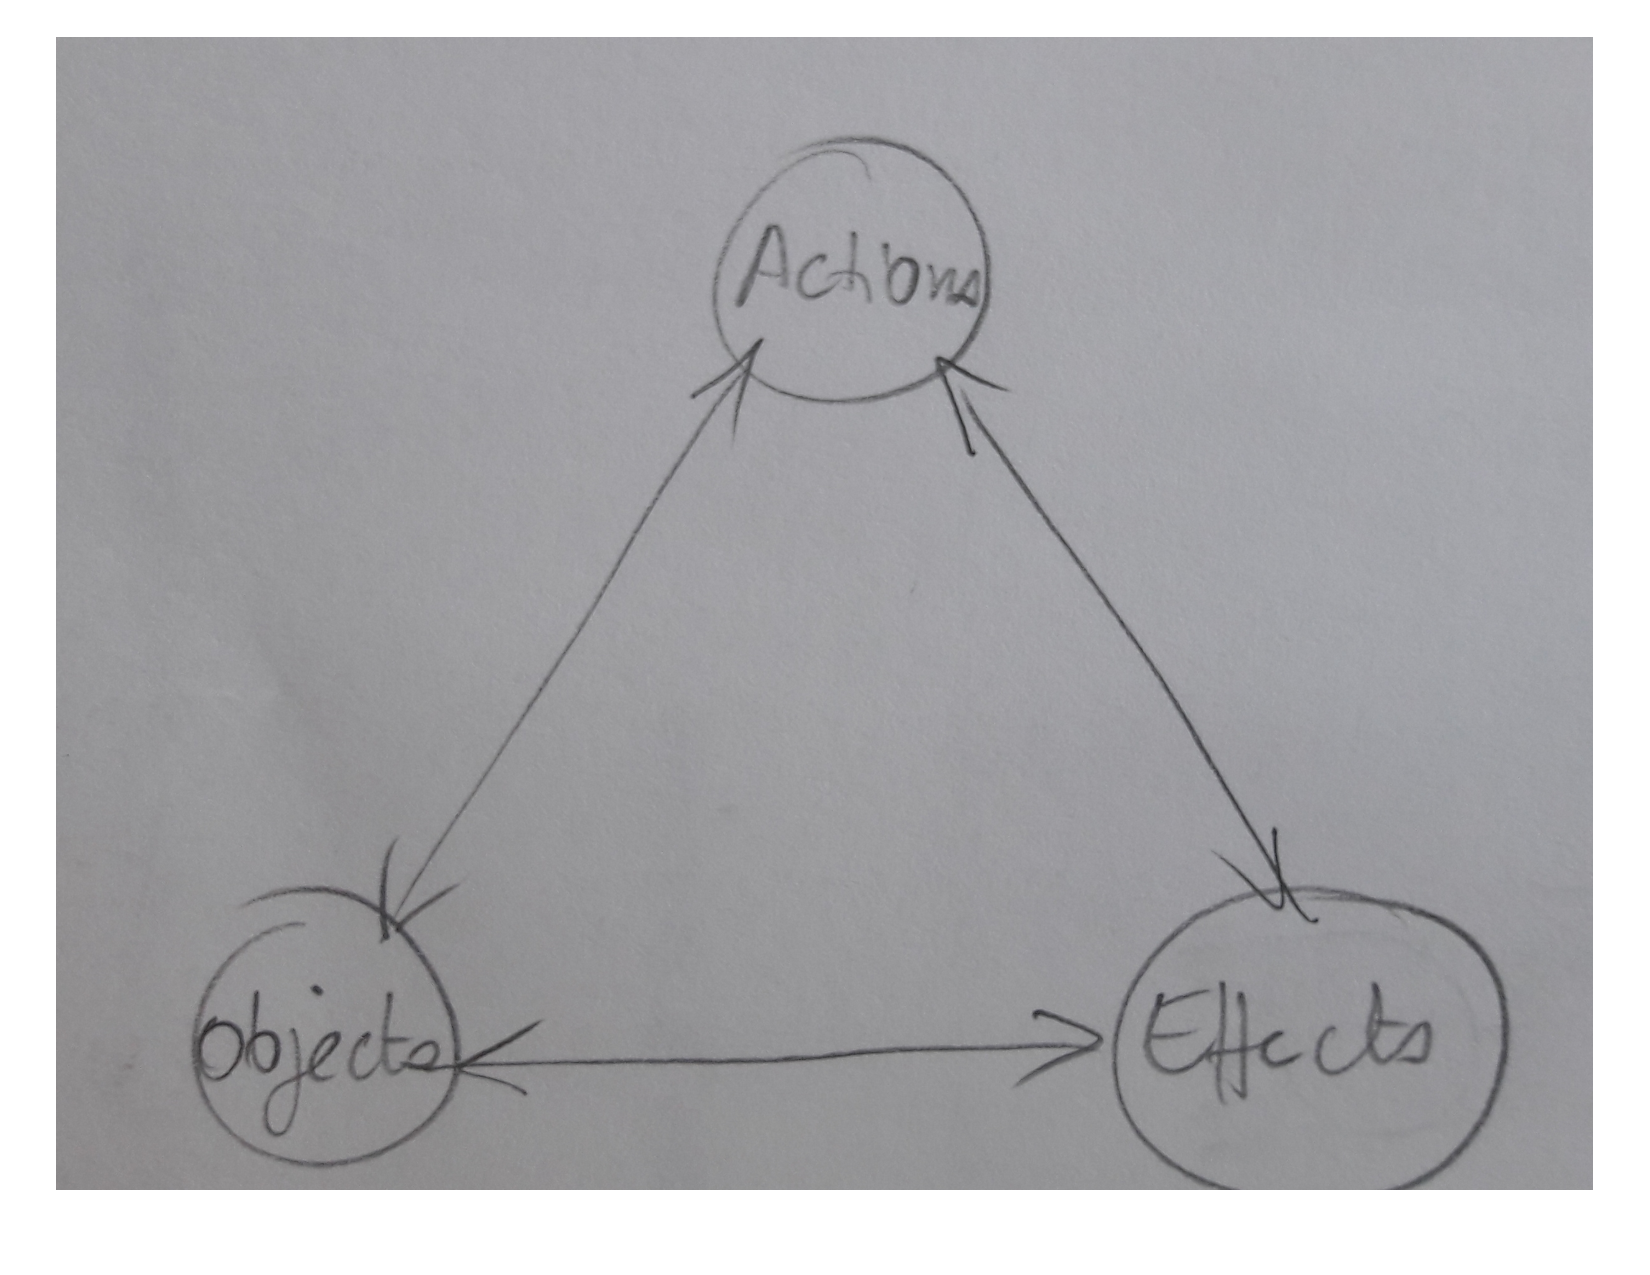
\includegraphics[width=.4\textwidth]{figures/affordances}
% 	\label{fig:affordances}
% 	\caption{Relationship between Actions, Ojects and Effects. \textit{To draw}}
% \end{figure}

\begin{figure}[!h]
\centering
  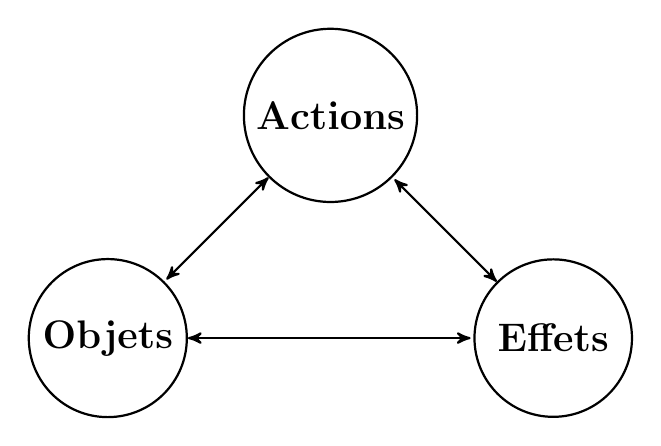
\begin{tikzpicture}[->,>=stealth',shorten >=1pt,auto,node distance=4cm,
                  thick,main node/.style={circle,draw,minimum size=20mm,font=\Large\bfseries}]

    \node[main node] (1) {Actions};
    \node[main node] (2) [below left of=1] {Objets};
    \node[main node] (3) [below right of=1] {Effets};

    % \path
    %   (2) edge node [below]{} (1)
    %   (3) edge node[right] {} (1)
    %       edge node[below] {} (2);
    \draw[<->] (1) edge  node[sloped, above] {} (2);
    \draw[<->] (2) edge  node[sloped, above] {} (3);
    \draw[<->] (3) edge  node[sloped, above] {} (1);
  \end{tikzpicture}

  \label{fig:affordances}
	\caption{Relation entre Objets, Actions et Effets.}

\end{figure}




%% Boostrapping
\subsubsection{Boostrapping}
Meltzoff et al. explained in \cite{EDP:EDP157} that infants do not know a priori what muscle movements achieve a particular state of organ relations. The authors call that process body babbling, directly inspired from babbling when infants experiment vocal sounds. In short, they explain that infants do repeated moves as a game. Eventually, after a certain amount of time and repetitions, infants would learn the relation between the moves they perform and theirs effects. That concept was reused in developmental robotics. Indeed, for a robot, learning affordances requires to interact with the environment throught an exploration stage, which corresponds to babbling. Several heuristics exist to perform that exploration.




%% Motor babbling
\subsubsection{Babillage sensorimoteur}
Une première approche naïve consiste à utiliser des mouvements aléatoires. Cette approche est la plus simple à implémenter mais elle peut générer un nombre important de mouvements qui ne produisent pas de contact avec les objets.

Une seconde approche est présentée dans dans \cite{Maestre2015} dans lequel Maestre et al. décrivent l'utilisation de Novelty Search, une algorithme évolutionnaire, afin de générer des trajectoires visant à maximiser l'exploration de l'environment. Les résultats montrent que les trajectoires permettant de toucher les objets sont davantage privilégiées au fur et à mesure des générations.




%% Intrinsic motivations
\subsubsection{Motivations intrinsèques}
Une troisième approche réside dans les motivations intrinsèques. Ce concept a été décrit par Ryan et Deci, puis par Hull et plus tard formalisé en modèles computationnels par Oudeyer et Kaplan dans \cite{10.3389/neuro.12.006.2007}. Les motivations intrinsèques permettent d'explorer progressivement l'environnement en favorisant une spécialisation progressive des modules. La curiosité est davantage favorisée au profit de la recherche de la performance. Ce concept est utilisé en robotique et spécifiquement en robotique développementale.

TODO : Définition de motivations intrinsèques, extrinsèques, internes et externes. Equivalent à la Curiosité.


% A third approache resides in intrinsic motivations, a concept described by Ryan and Deci, then by Hull and later formalized in computational models by Oudeyer and Kaplan \cite{10.3389/neuro.12.006.2007}. Intrinsic motivations allow to explore the environment by progressively specializing. Concept reused in robotics and especially in developmental robotics.

Context: The ability to perform in an open-ended environment and to build on previously acquired knowledge to quickly adapt to changes and unknown situations is key to building
multi-purpose assistive robots which can be helpful in a wide range of realistic situations.

%% Cognitive Developmental
Cognitive Developmental robotics is a promising approach to create robots with higher cognitive functions as shown in \cite{Asada2009} by Asada et al.





%% Use of tools
\subsubsection{Utilisation d'outils}
Au delà des affordances, des recherches prometteuses se concentrent sur la manipulation d'outils. Dans \cite{Goncalves2014}, Gonçalves et al. proposent une approche intéressante pour apprendre les affordances visuelles d'objets ou d'outils. Dans cet article, un robot apprend les caractéristique visuelles d'objets et d'outils à l'aide de descripteurs visuels. De cette façon, ils montrent que le robot est capable de réaliser une action spécifique ou d'obtenir un résultat désiré. L'utilisation des descripteurs visuels permet au robot de généraliser avec des objets inconnus.

% Beyond affordances, promising researches focused on tool usage. In \cite{Goncalves2014}, Gonçalves et al. proposed an interesting approach to learn visual affordances of objects and tools. In that paper, a robot learned visual features of objects and tools by using visual descriptors. Then, they show that the robot is able to perform a specific action or obtain a desired result. The use of visual descriptors allow the robot to generalize with unknown objects.

%% Bayesian network
\subsubsection{Réseaux bayésiens}
Une fois que le babillage sensorimoteur a été réalisé, les relations entre les objets, actions et effets nécessitent d'être modélisées. Les réseaux bayésiens constituent une méthode pour réaliser cela. Ce sont des modèles probablistes qui représentent les relations entre leurs variables. Dans \cite{4456755}, Montesano et al. présentent un modèle de réseau bayésien qui permet d'apprendre des affordances concernant des objets.

Our work focused on improving the paper of \cite{Ugur2011}. In that paper, Ugur \textit{et al}.
described a system that allows a robot to learn goal emulation by using learnt affordances. In order to that, the robot follows an observation stage then an imitation stage.

- bootstrap object-oriented behavior
- discover object in an unknown environment




% \subsection{Related work}

% Ce stage de fin d'études l'a été dans le cadre du projet DREAM, débuté en 2015. Ce projet implique 5 partenaires académiques: UMPC/CNRS (coordinateur), ENSTA ParisTech, Universidade da Coruña, Vrije Universiteit Amsterdam et Queen Mary University of London. Ces différents acteurs ont différents rôles au sein du projet DREAM. See waves.

% \`A l'issue du projet DREAM, les différents modules doivent permettre de constituer un ensemble.
% % At the end of the DREAM project, the different modules are aimed at be linked together.

% Our work is directly based on actual PhD student's work on learning affordances inspired from motor babbling.

% Linkedin: "The main goal of this thesis is the autonomous creation by a robot of a minimal directory of concepts related to its morphology, its environment, and the accomplished tasks executed. The robot must be able to build and update its internal world model through interactions with its environment (cognitive bootstrapping). This work follows the approach proposed in developmental robotics, inspired by the development of the infants, where abstract concepts are created progressively based on the sensori-motor capabilities of an agent.

% Executed in an iterative loop, a dataset is created by the robot through the babbling of its environment; some candidate world models are defined based on the data gathered; and a new dataset is created, in order to discriminate these models, improve them and generate new simpler ones."




\section{Notre travail}

% \epigraph{Artificial intelligence is the science of making machines do things that would require intelligence if done by men.}{\textit{Marvin Minsky}}




\subsection{Environnement}
 
Durant notre stage, l'environnement de travail était composé de différents composants. ROS est un framework flexible pour contrôler un robot. Il comporte différents outils, bibliothèques de fonctions\footnote{http://www.ros.org/}.

Gazebo\footnote{http://gazebosim.org} est un simulateur. La figure \ref{fig7} donne un aperçu d'une simulation lancée avec Gazebo.

MoveIt!\footnote{http://moveit.ros.org} est un simulateur open source conçu pour la manipulation de robots et inclut de nombreux composant de motion planning, manipulation, perception 3D, cinématique, conrôle et navigation. Ce simulateur permet de de développer facilement des applications robotiques complexes.

Dans le cadre du projet DREAM, l'ISIR bénéficie du robot Baxter\footnote{http://www.rethinkrobotics.com/baxter/tech-specs/} (voir figure \ref{fig:baxter}), c'est un robot développé par Rethink Robotic et utilisé à la fois à des fin industrielles et de recherche. Ce robot antropormorphique à 2 bras dispose de 2 fois 7 degrés de liberté et de multiples senseurs\footnote{http://sdk.rethinkrobotics.com/wiki/Hardware\_Specifications}.

\begin{figure}
	\centering
	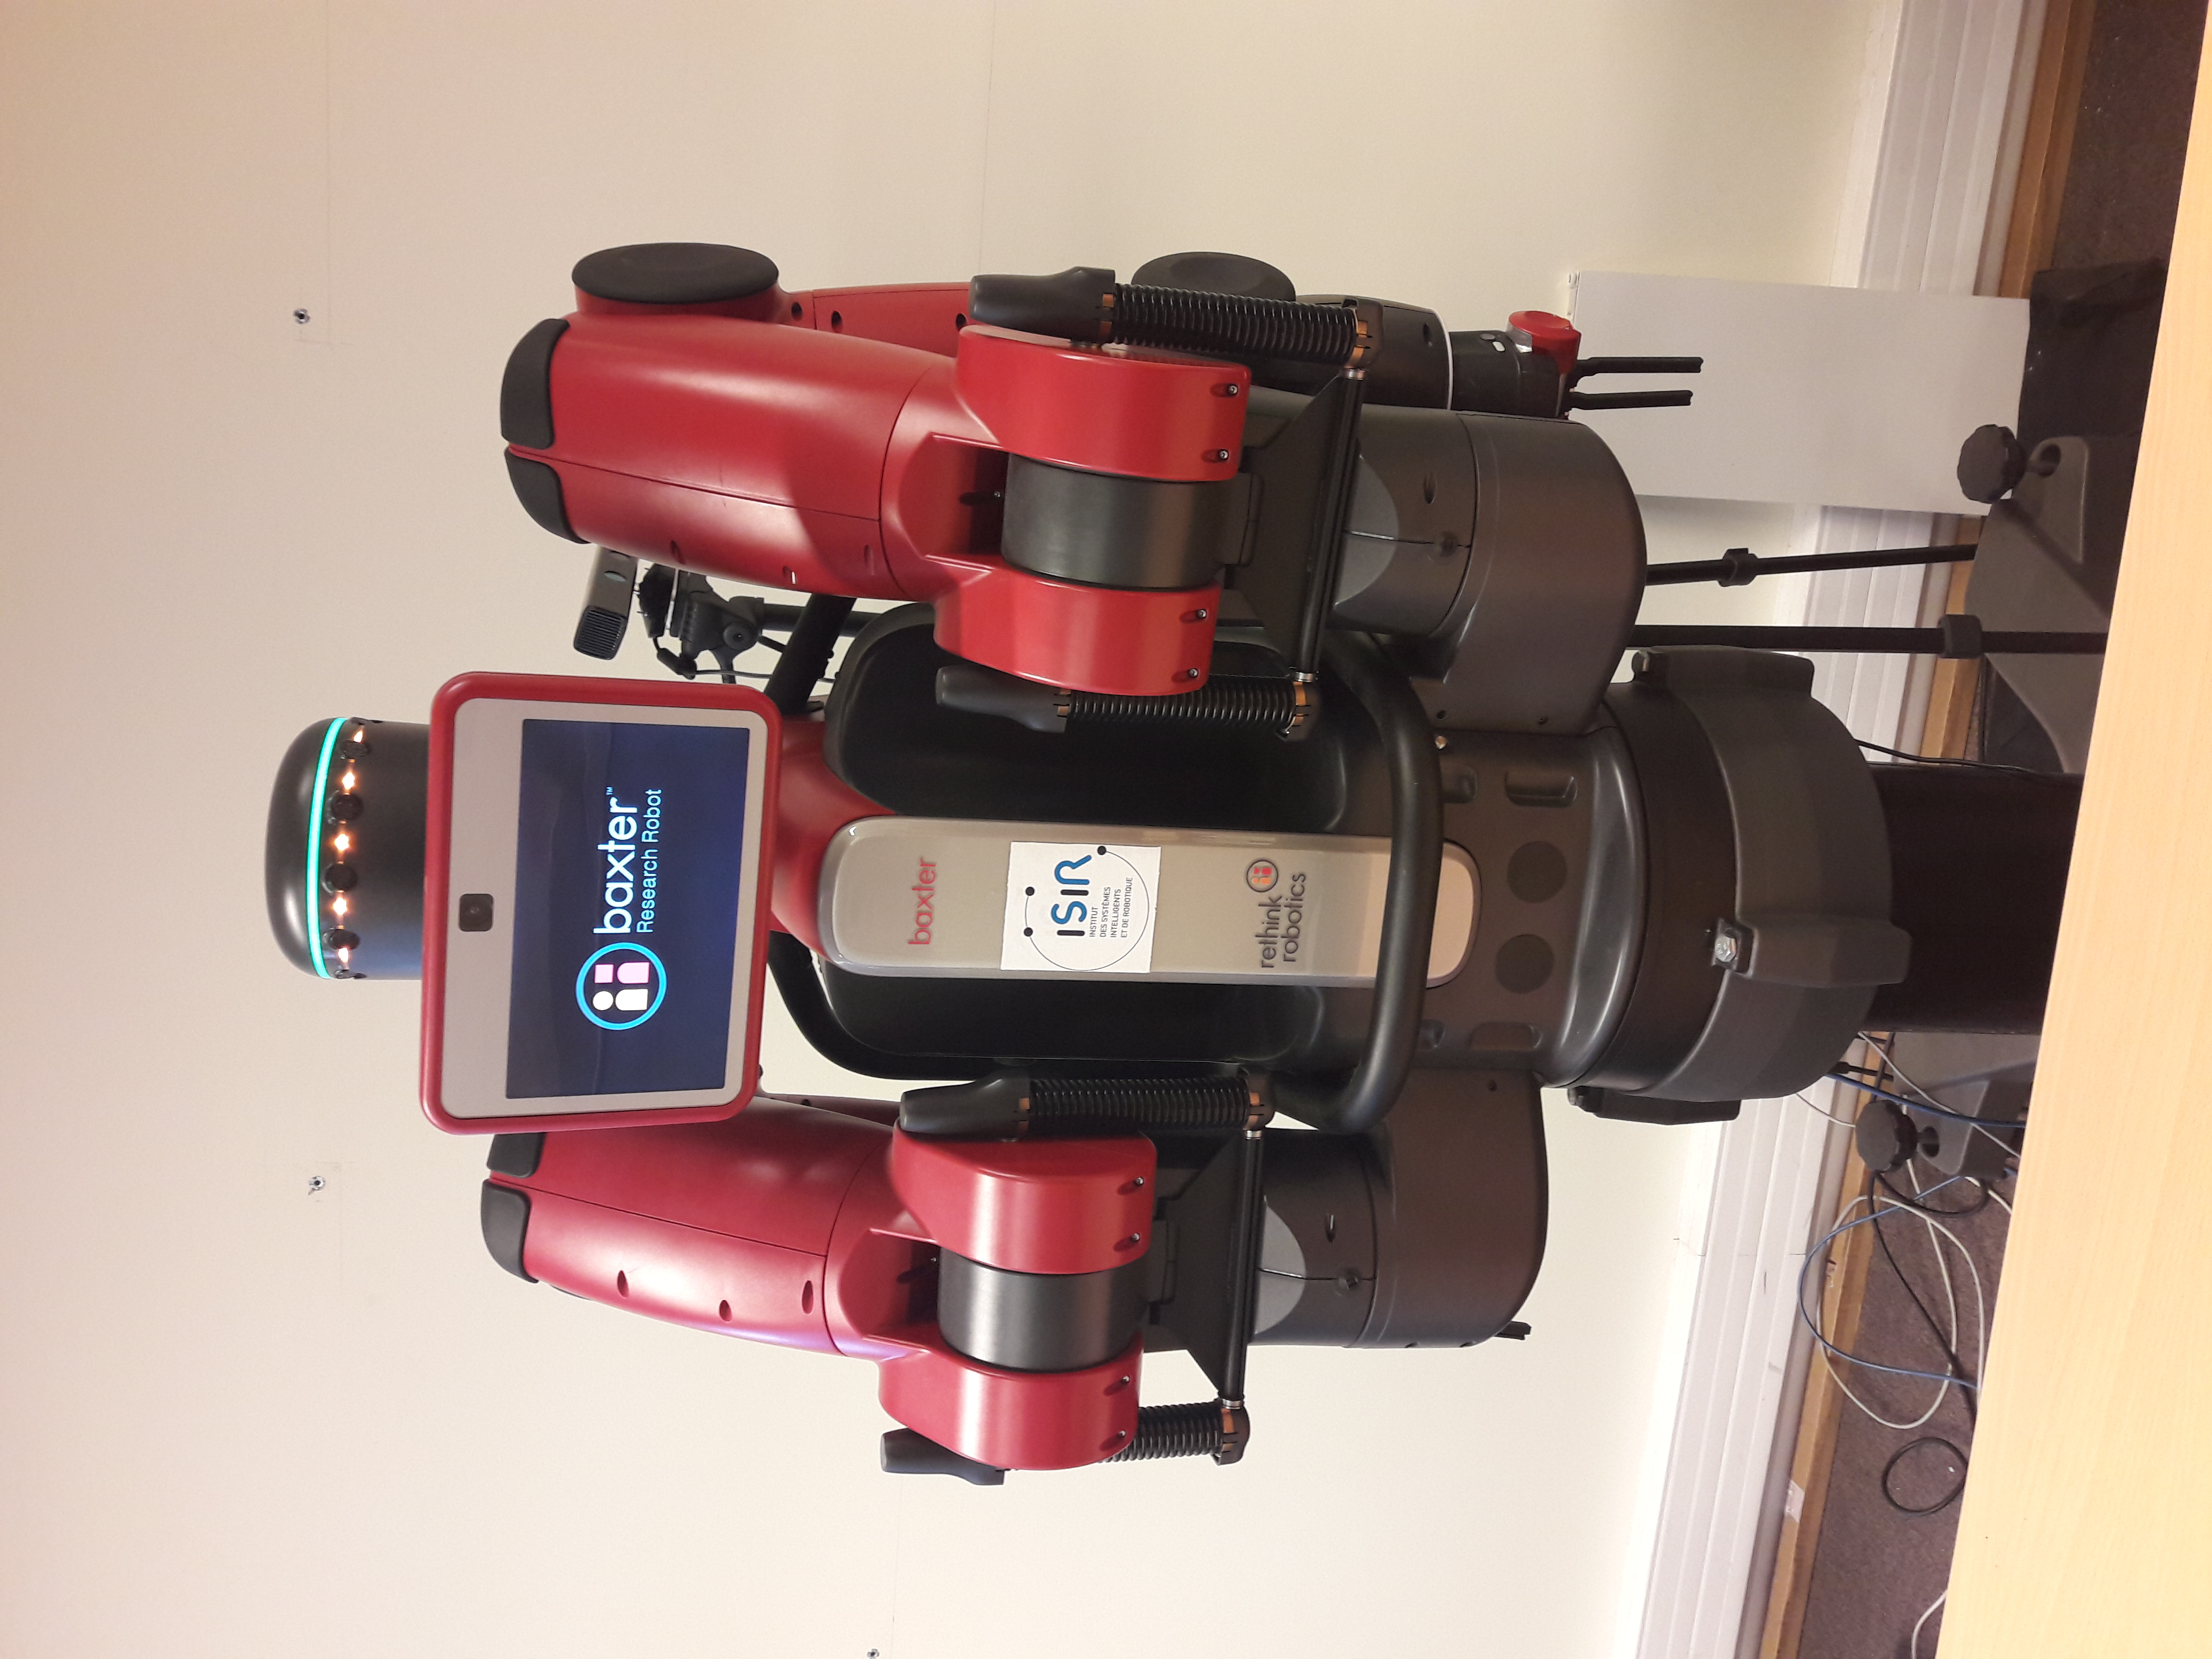
\includegraphics[angle=-90,width=.4\textwidth]{figures/baxter}
	\label{fig:baxter}
	\caption{Le robot Baxter de Rethink Robotics utilisé à l'ISIR.}
\end{figure}

% \begin{figure}
% 	\centering
% 	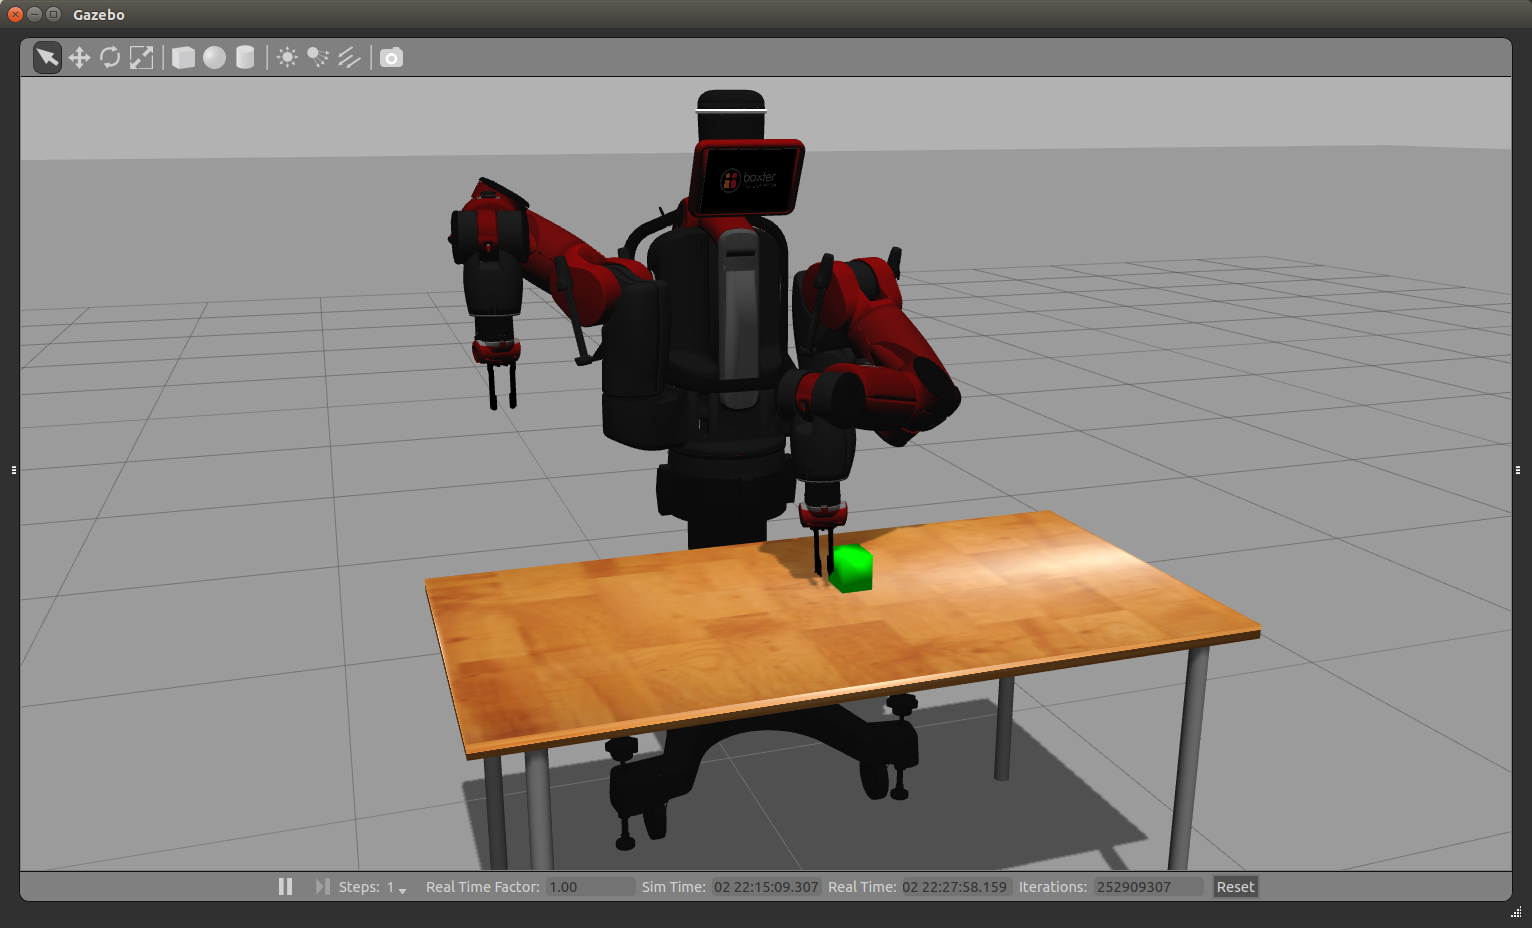
\includegraphics[width=\textwidth]{figures/gazebo}
% 	\label{fig:gazebo}
% 	\caption{Gazebo simulator}
% \end{figure}




\subsection{Discrétization adaptative}



\subsubsection{Previous works}

Notre travail se base en partie sur les travaux d'un doctorant, intégré dans le projet DREAM, et portant sur la découverte des affordances. Dans cette première étape, le nombre d'actions disponibles et connues par le robot est arbitrairement paramétré (4 ou 8) (\textbf{Gauche}, \textbf{Droite}, \textbf{Haut}, \textbf{Bas}). Voir figure~\ref{fig:trajectories}.

\begin{figure}
	\centering
	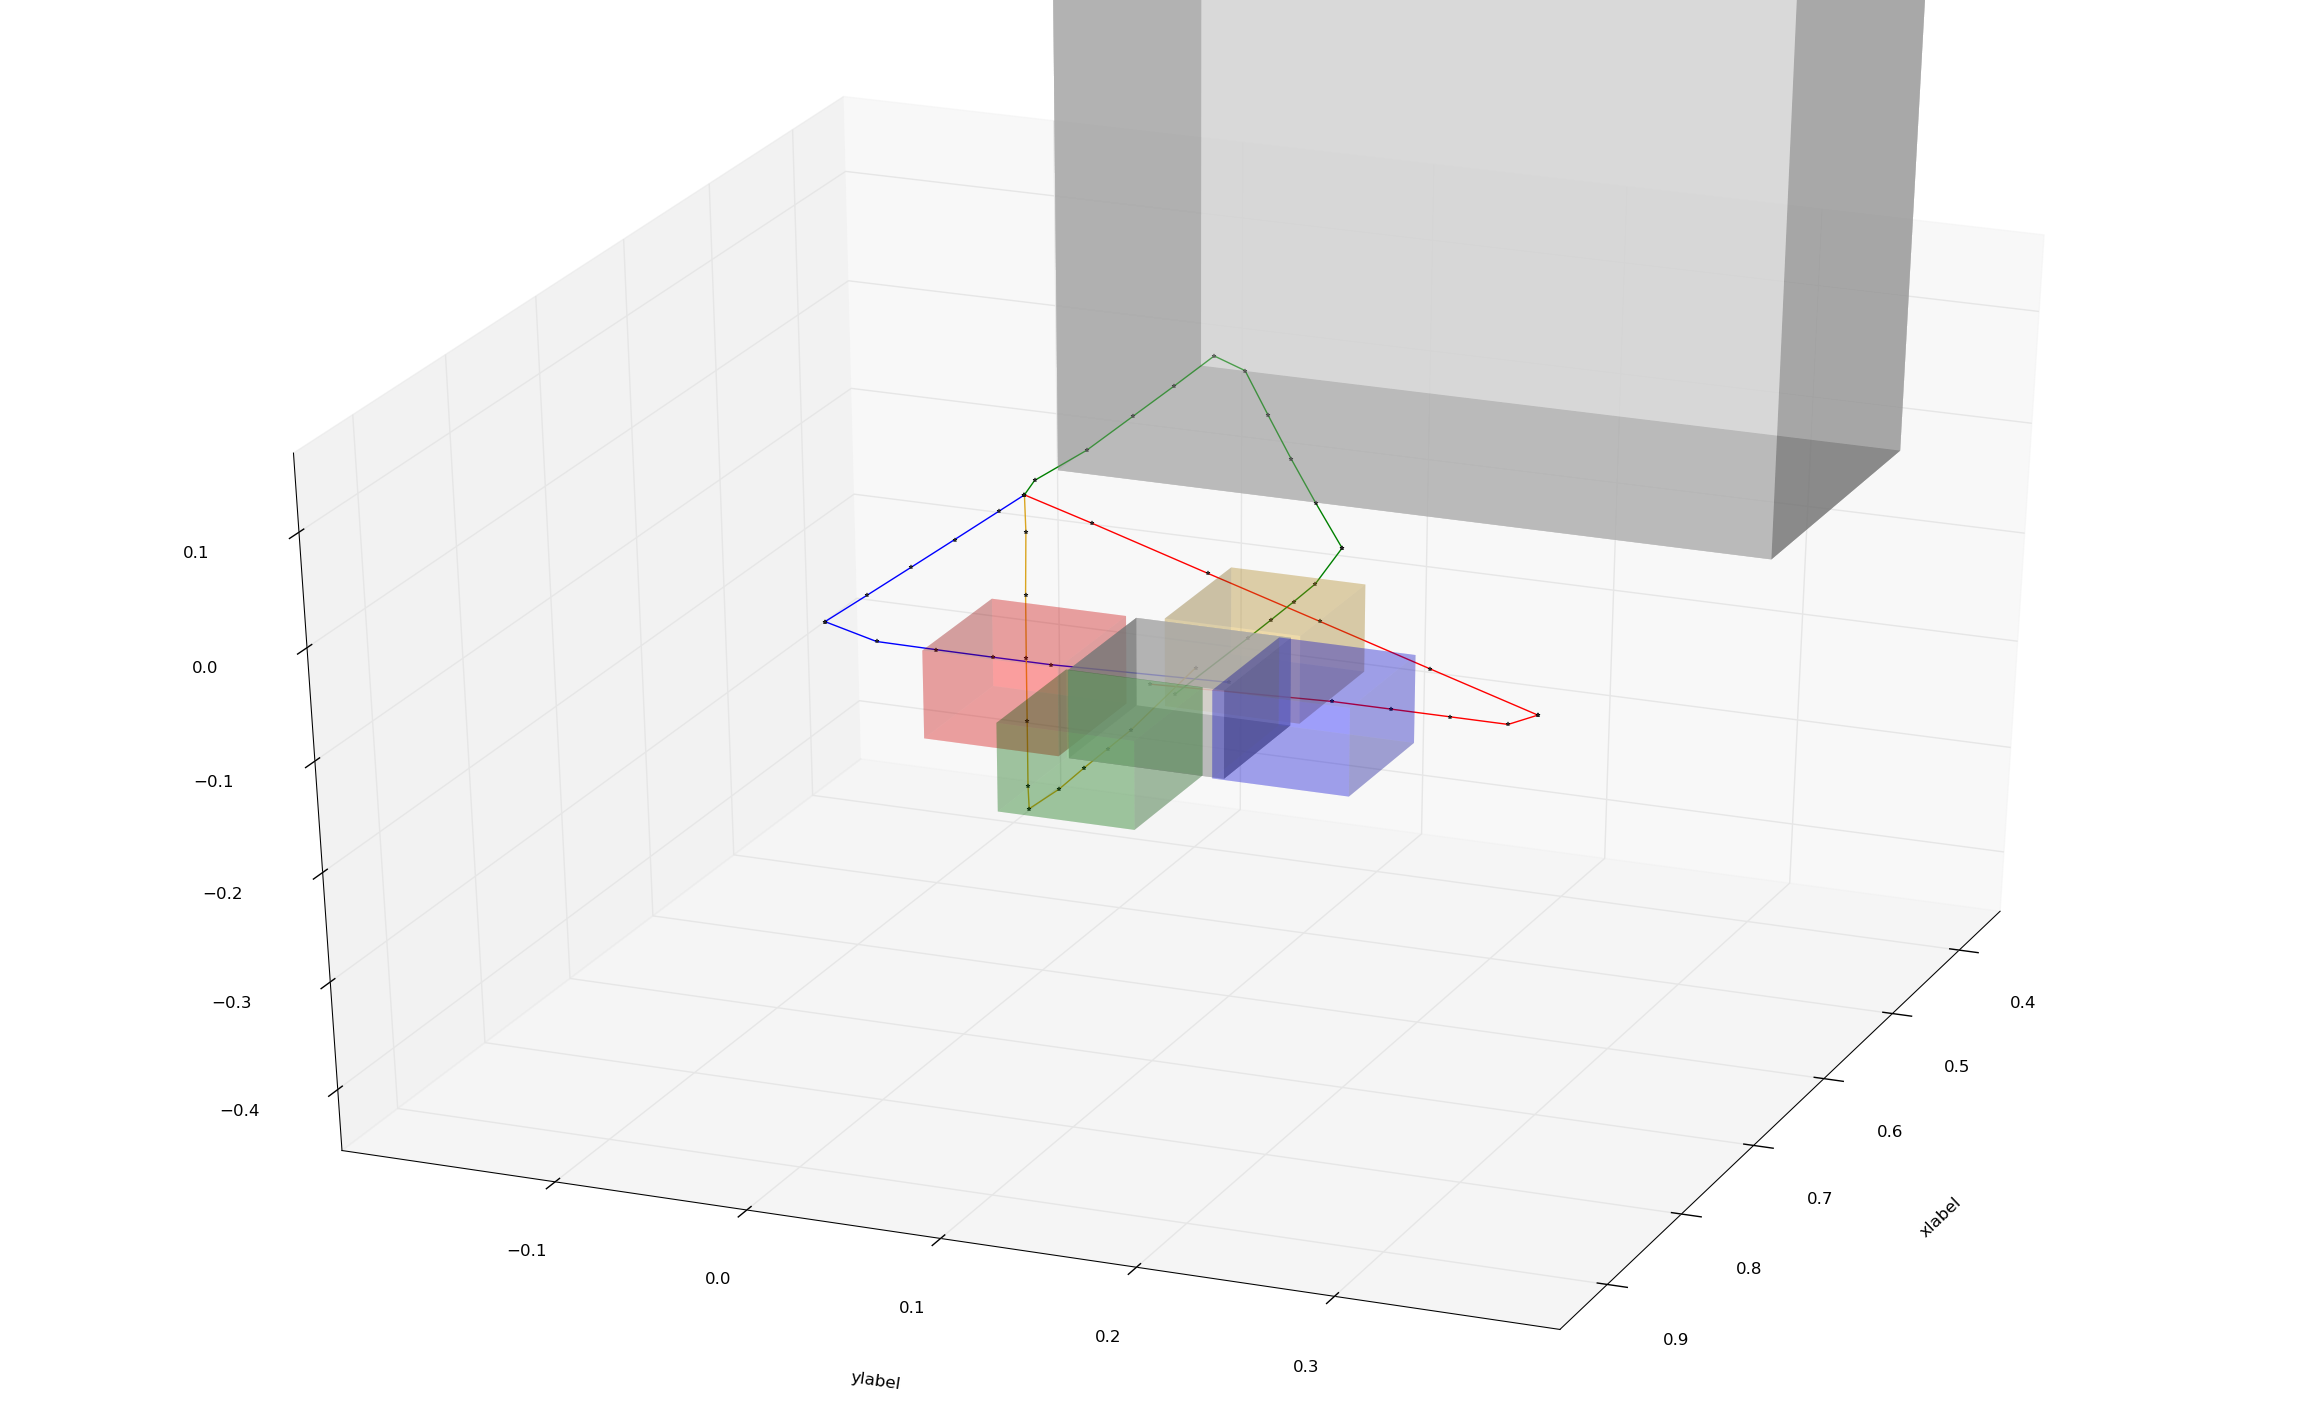
\includegraphics[width=0.5\textwidth]{figures/trajectories}
	\caption{Différentes trajectoires réalisées par le robot (représenté par le volume gris). La position initiale de l'objet est représentée par le cube gris au milieu. Chqaue cube coloré correspond au mouvement de la même couleur (par exemple, le cube rouge est la position finale du cube gris après avoir poussé par l'effecteur du robot suivant la trajectoire rouge).}
	\label{fig:trajectories}
\end{figure}

En raison de la nécessesité de généraliser, il n'est pas possible de laisser une telle valeur arbitraire. Pour pallier à ce problème, la première étape de notre stage a porté sur l'accomplissement d'une discrétisation adaptative de l'environnement. L'idée générale est de laisser le robot découvrir lui-même les différentes actions réalisables sans en spécifier le nombre. Pour arriver à cela, le clustering est utilisé afin de distinguer les différentes actions. 

X-means algorithm\cite{Pelleg:2000:XEK:645529.657808}, based on k-means, was used at the beginning. Basically, X-means is a k-means algorithm's generalization, which finds itself the best value for $k$.




Dans Ugur, l'algorithme de clusterisation \textit{X-means} est utilisé pour clusteriser les effets. Mais pas paramètrable. Cf long abstract (v1, v2, v3).

% \begin{figure}
% 	\centering
% 	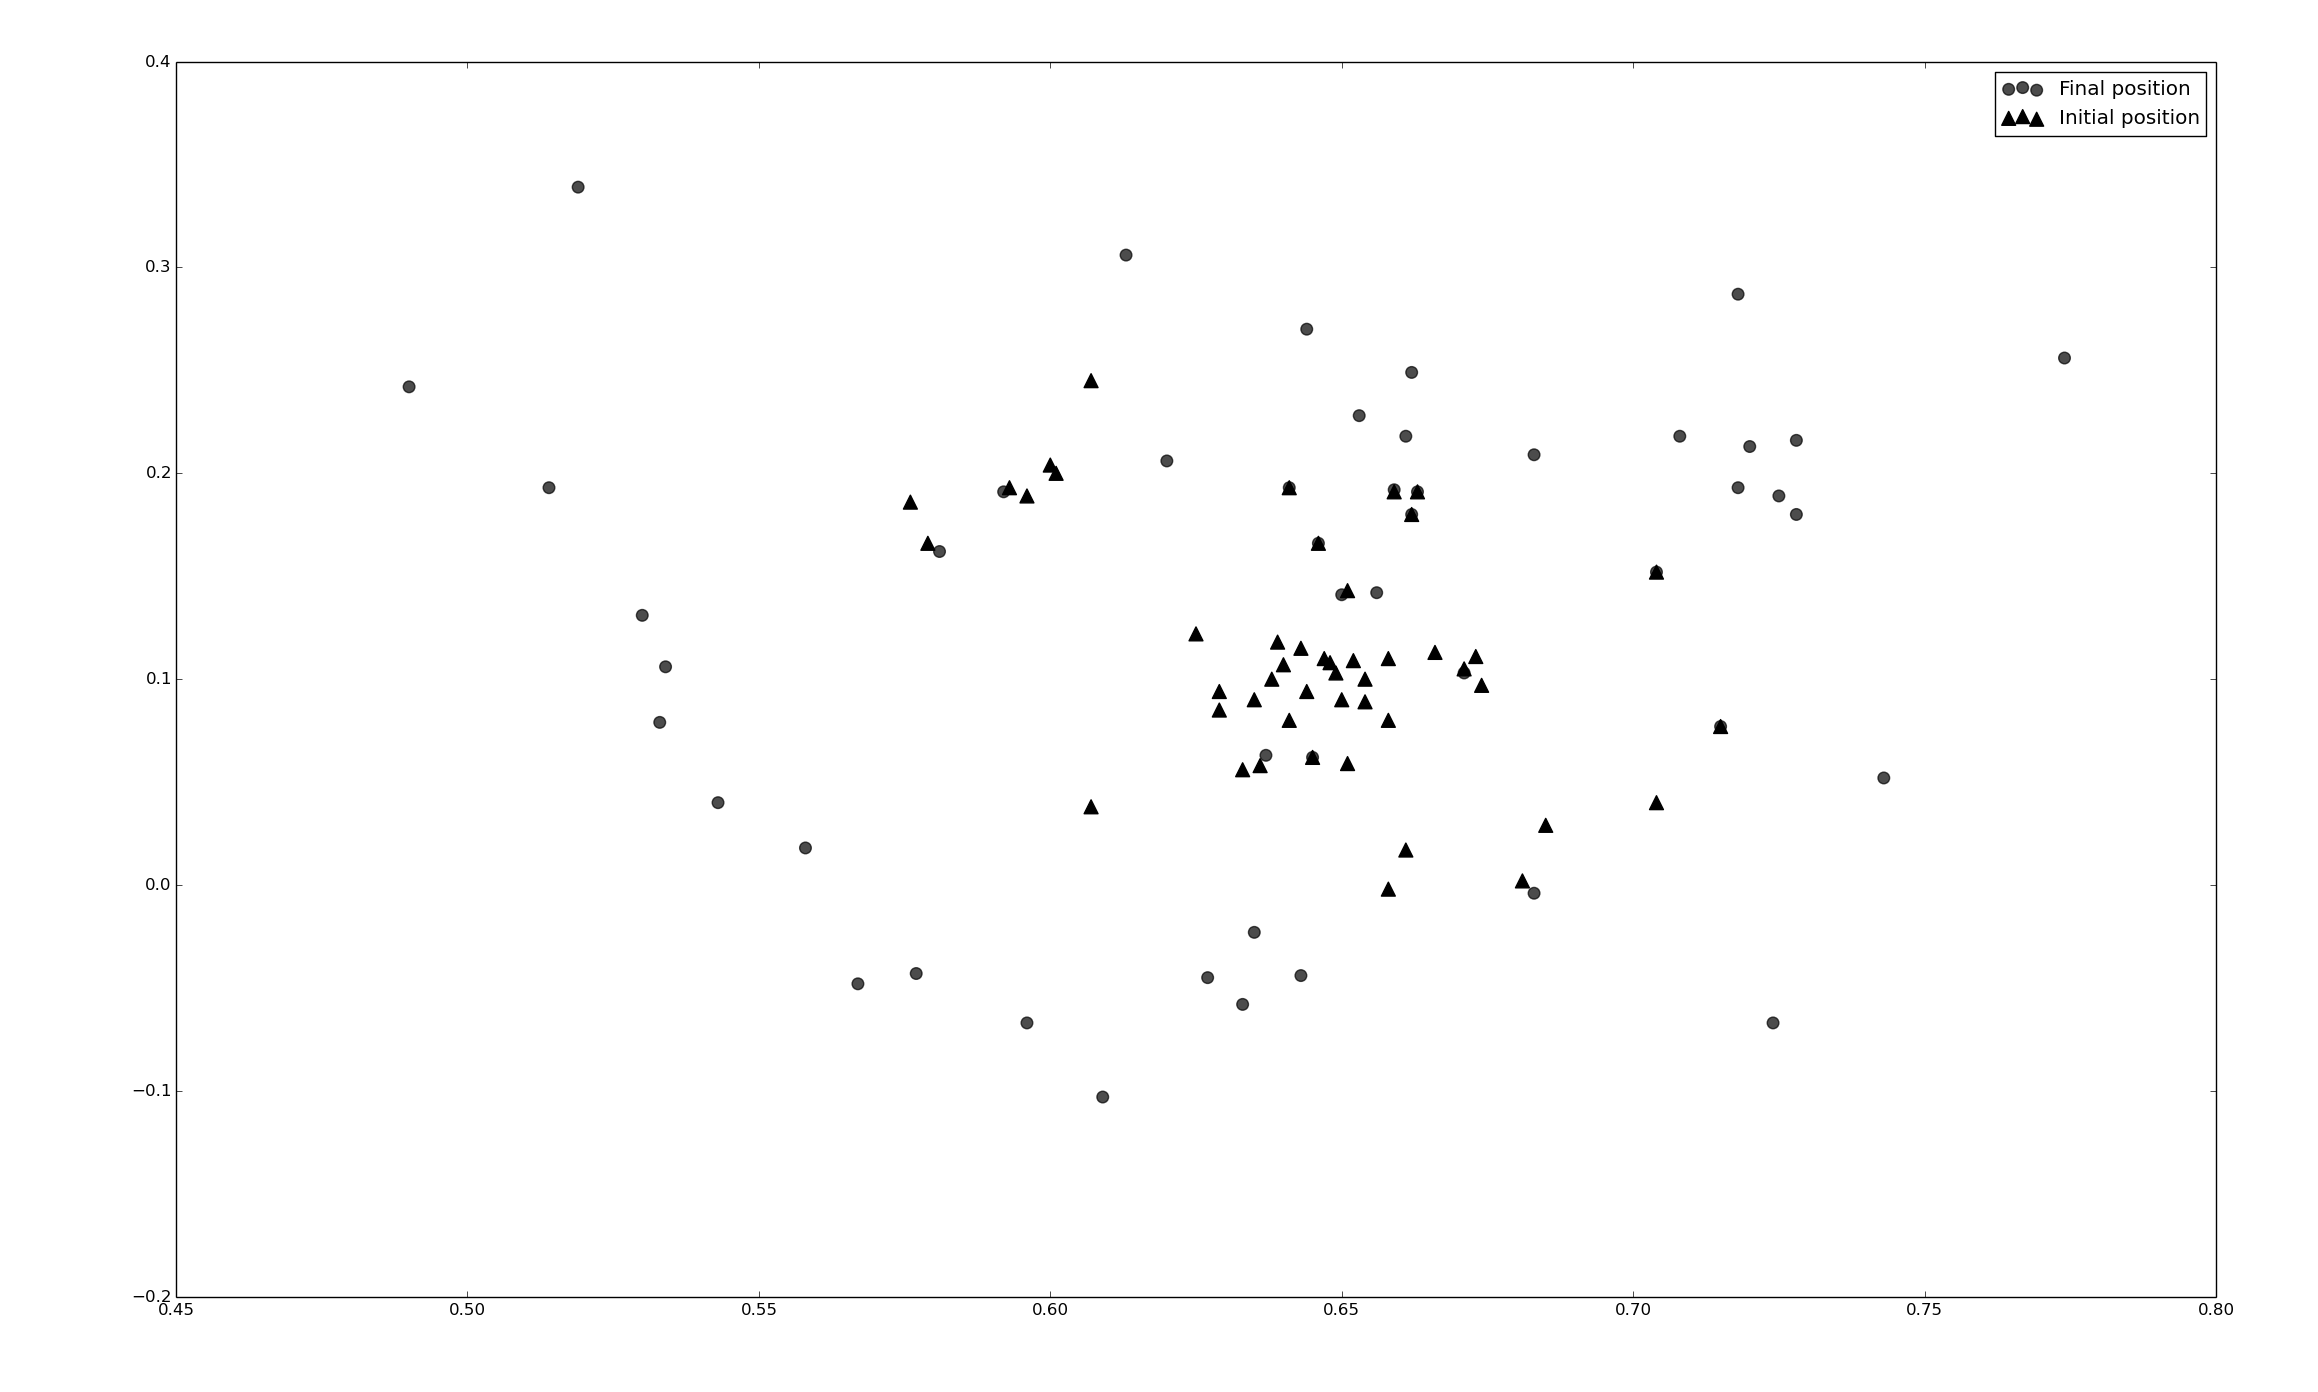
\includegraphics[width=\textwidth]{figures/before_offset_correction.png}
% 	\label{fig:plot_before}
% 	\caption{Original dataset}
% \end{figure}
%
% \begin{figure}
% 	\centering
% 	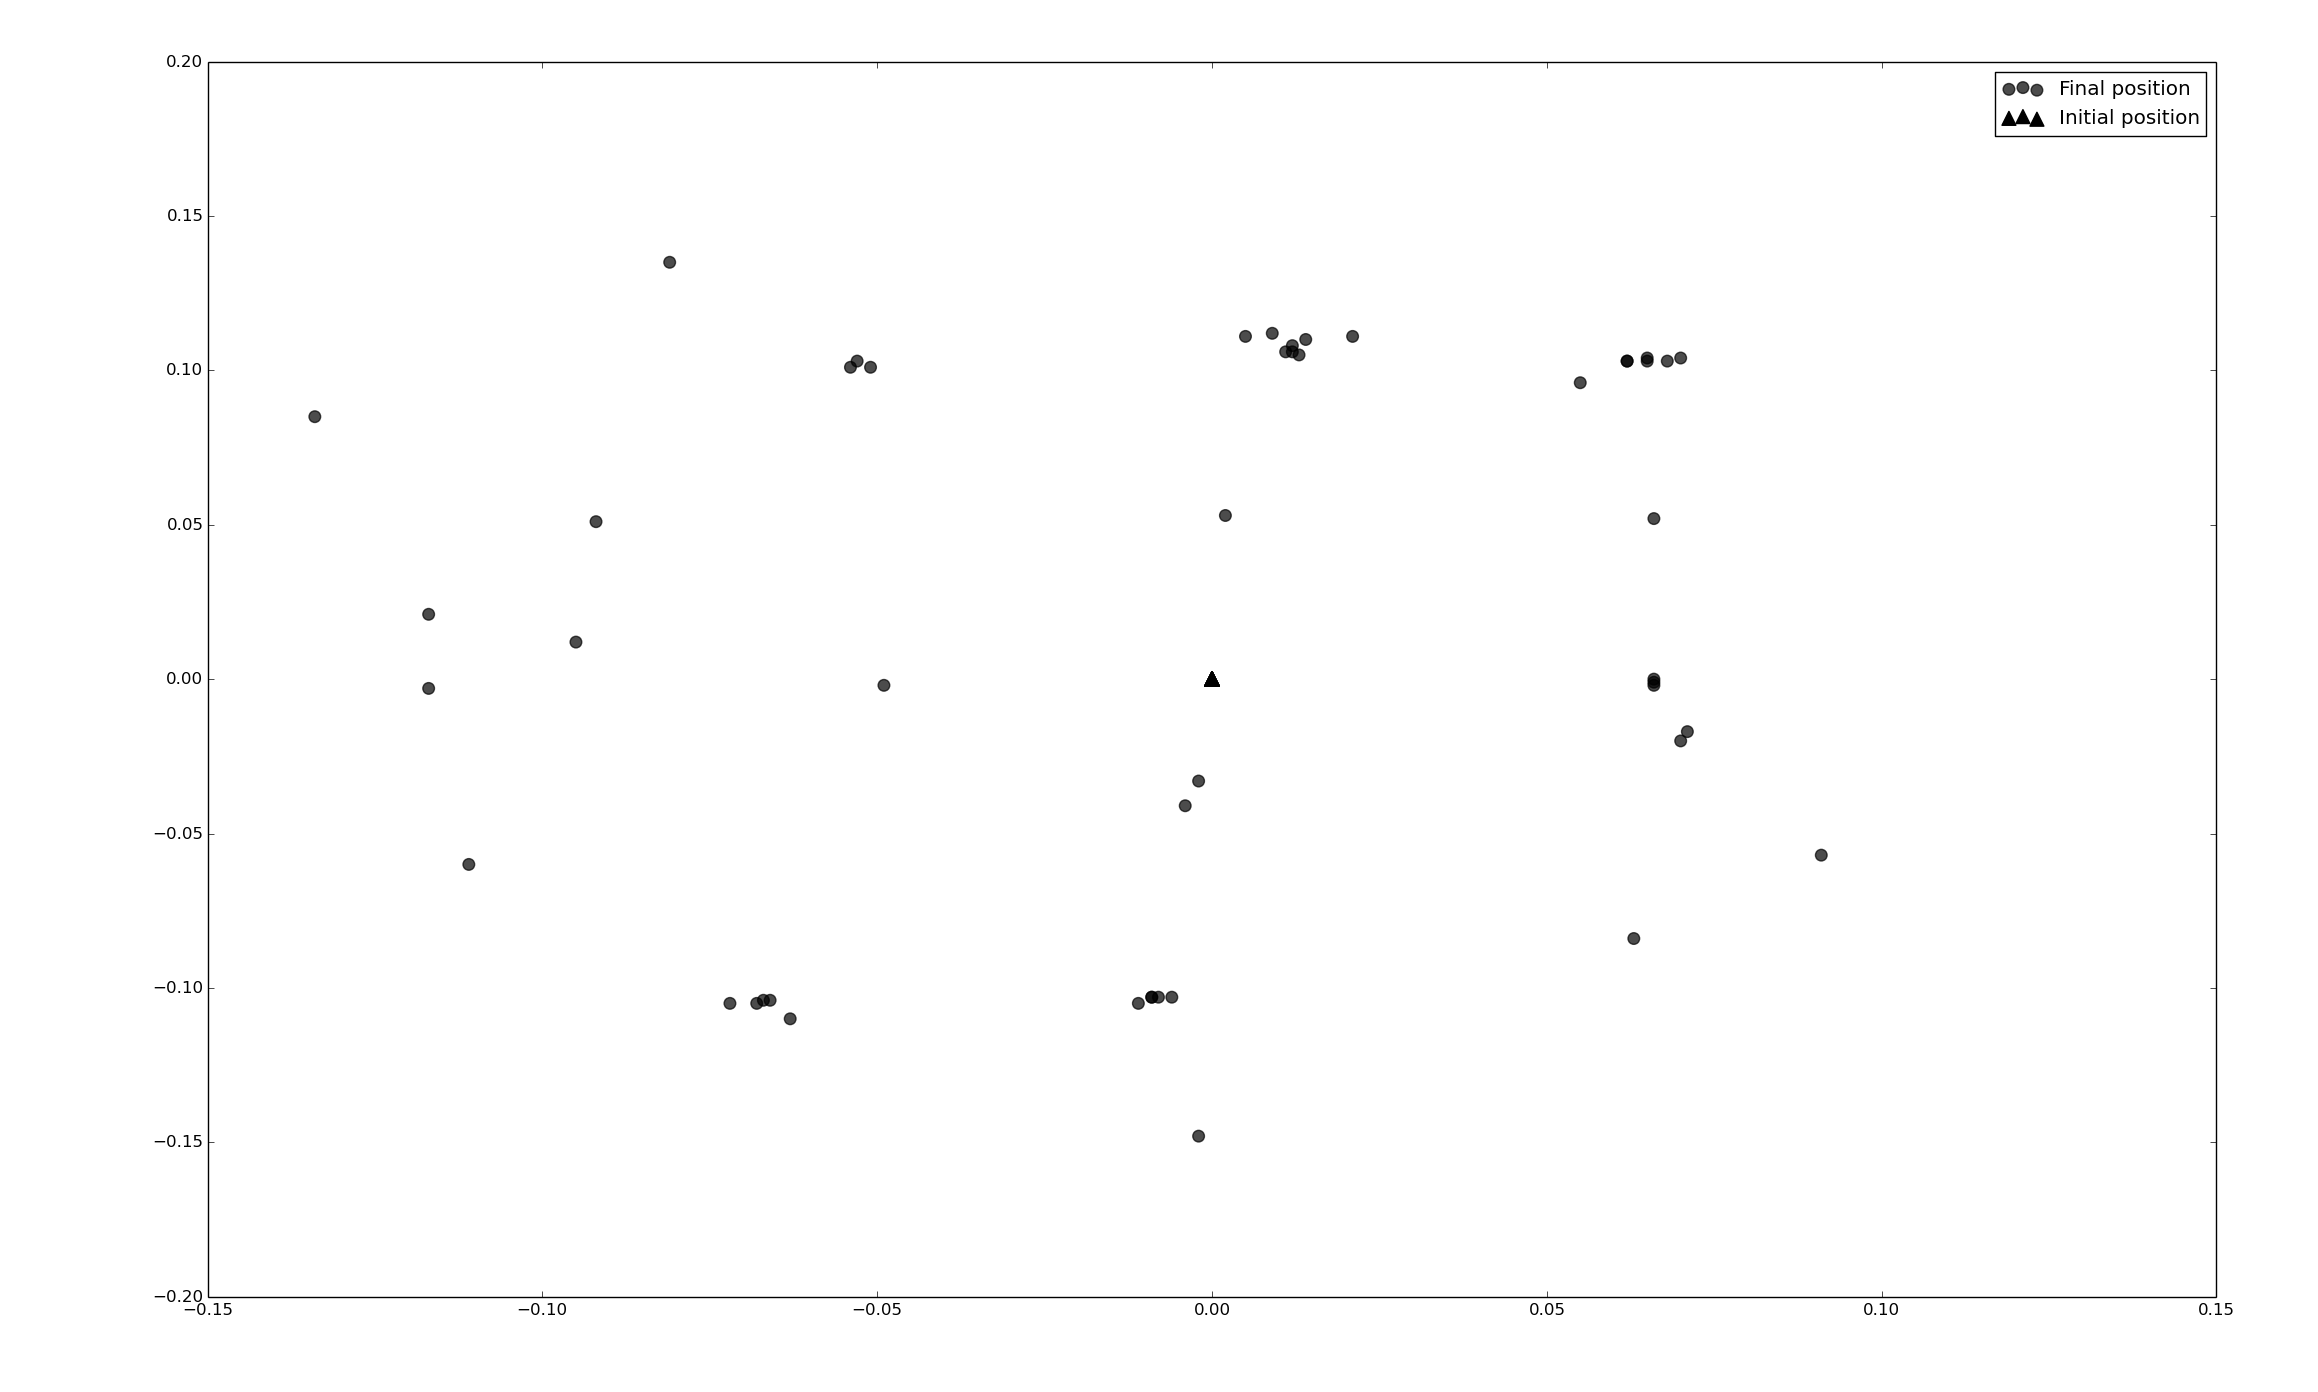
\includegraphics[width=\textwidth]{figures/after_offset_correction.png}
% 	\label{fig:plot_after}
% 	\caption{Trajectories where initial points' offset are corrected}
% \end{figure}



\subsubsection{Algorithmes de clustering}

En nous basant sur \cite{Xu2015}, \cite{Andreopoulos2009}, \cite{Fahad2014} et \cite{Sajana2016}, nous avons réalisé une synthèse des algorithmes de clustering les plus communément utilisés, groupés en catégories (c.f. Annexe pour plus de détails). Afin de filtrer et sélectionner les algorihtmes les plus pertinents, nous avons choisi des critères non arbitraires. En se référant à la généralisation mentionnée ci-dessus, un premier critère concerne la nécessité de ne pas fournir le nombre attendu de clusters en paramètre. En effet, puisque le système doit être capable de trouver lui-même le nombre correct d'actions. Un second critère concerne la possibilité de travailler avec de nombreuses dimensions et un troisième concerne la disponibilité d'une implémentation en Python ou C{}\verb!++!. Les algorithmes ne satisfaisant pas à ces critères ont été rejetés.

Sur la centaine d'algorithmes de clustering existants, 7 ont été retenus lors de cette première phase : X-means\textsuperscript{1}, Affinity Propagation\textsuperscript{1}, DBSCAN\textsuperscript{2}, HDBSCAN\textsuperscript{2}, OPTICS\textsuperscript{2}, Mean-Shift\textsuperscript{2} et Level Set Tree. (1) correspondent à des algorithmes de partitionnement et (2) correspondent à des algorithmes basés sur la densité.

% Based on \cite{Xu2015}, \cite{Andreopoulos2009}, \cite{Fahad2014} and \cite{Sajana2016}, we reviewed the most common algorithms used for clustering, grouped in categories (see annex for details). Non-arbitrary criteria were required for filtering algorithms. According to the generalization mentioned above, a first criterion concerns the requirement to pass the number of clusters as input parameter. Indeed, as the system should be able to find itself the correct number of actions. A second criterion concern the possibility to work with high dimensionality and a third one is the implemenation's availabily in Python or C++. Algorithms that did not suit to those parameters were discarded.

% The intuition behind that choice is based on the fact that the different categories of actions have roughly the same end position. In other terms, a \textbf{Left} action will end in the specific area for left actions. Hence, a large amount of space will be empty and will not contain any end positions. The points distribution would lead to focus on finding areas of high density. For that purpose, density-based algorithms exist.

% Afin de comparer les différents algorithmes, une série de tests a été réalisée avec 2 jeux de données différents : un dataset avec une distribution uniforme de points et un jeu de données généré en simulation.


% \begin{figure}
% 	\centering
% 	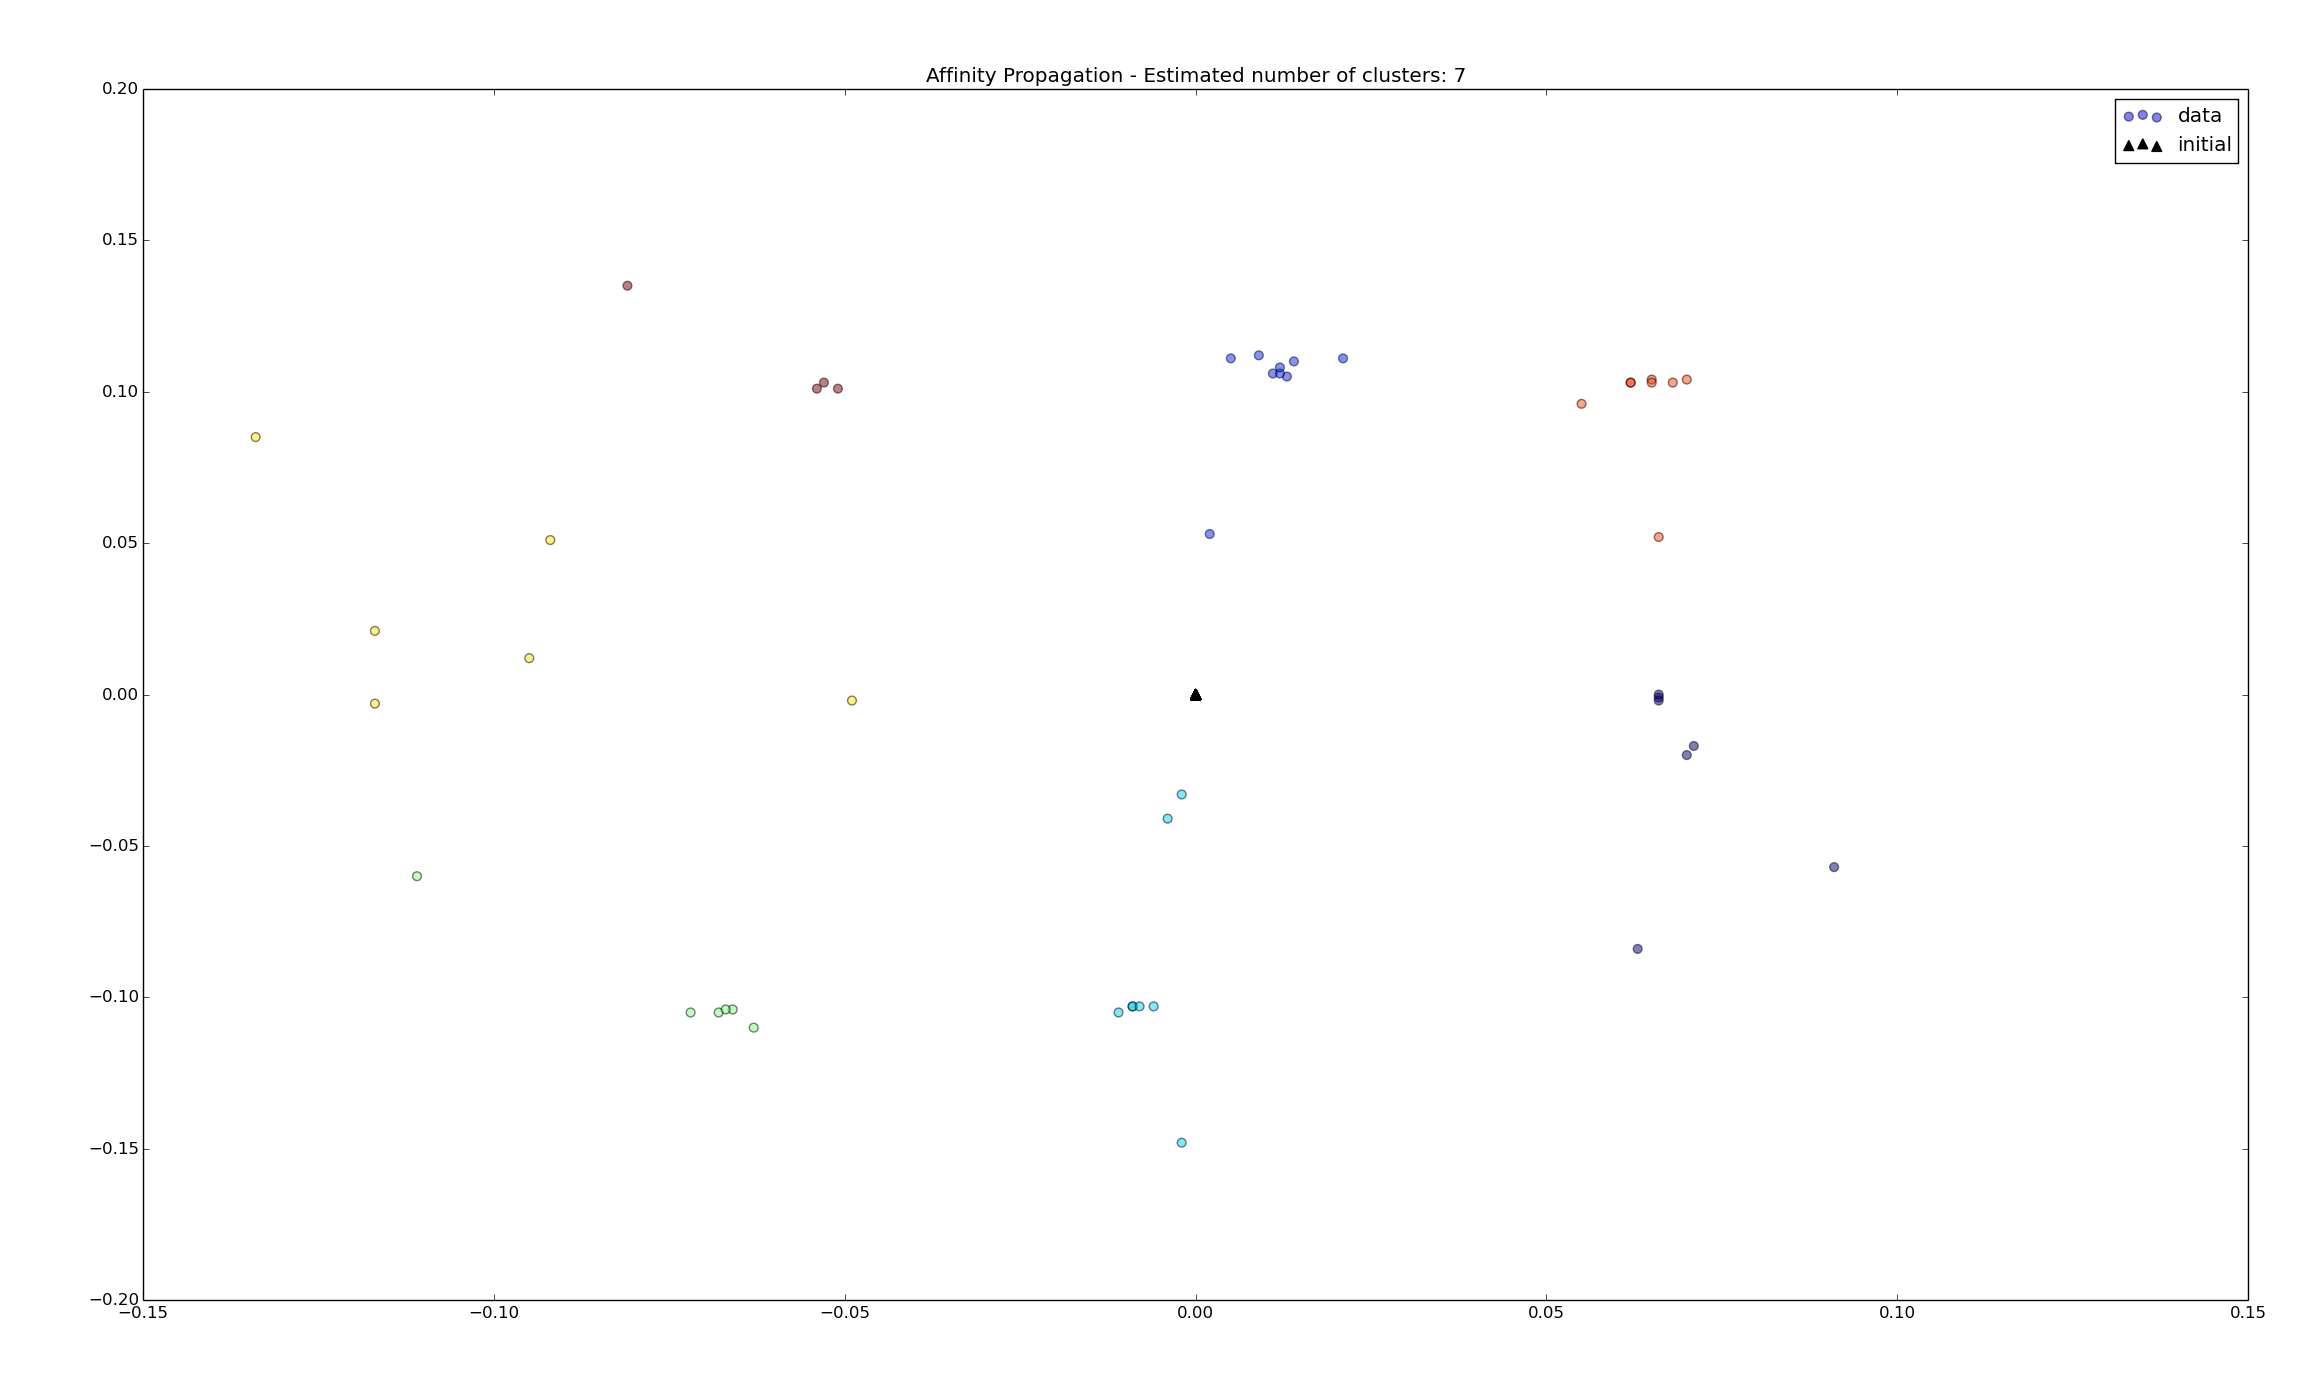
\includegraphics[width=\textwidth]{figures/clustering_results/AP}
% 	\caption{Clustering with Affinity Propagation. AP clusters correctly the dataset. Parameters are: \textit{damping=0.5, preference=-0.0095}}
% 	\label{fig:ap}
% \end{figure}

% Clustering results were very dependent on the dataset. For instance, in the Figure~\ref{fig:comparison}, the clusters are not perfect. Indeed, both clusters at bottom left (blue and yellow) should have been grouped into one cluster. That single cluster is, however, also difficult to predict for human.

% \begin{figure}
% 	\centering
% 	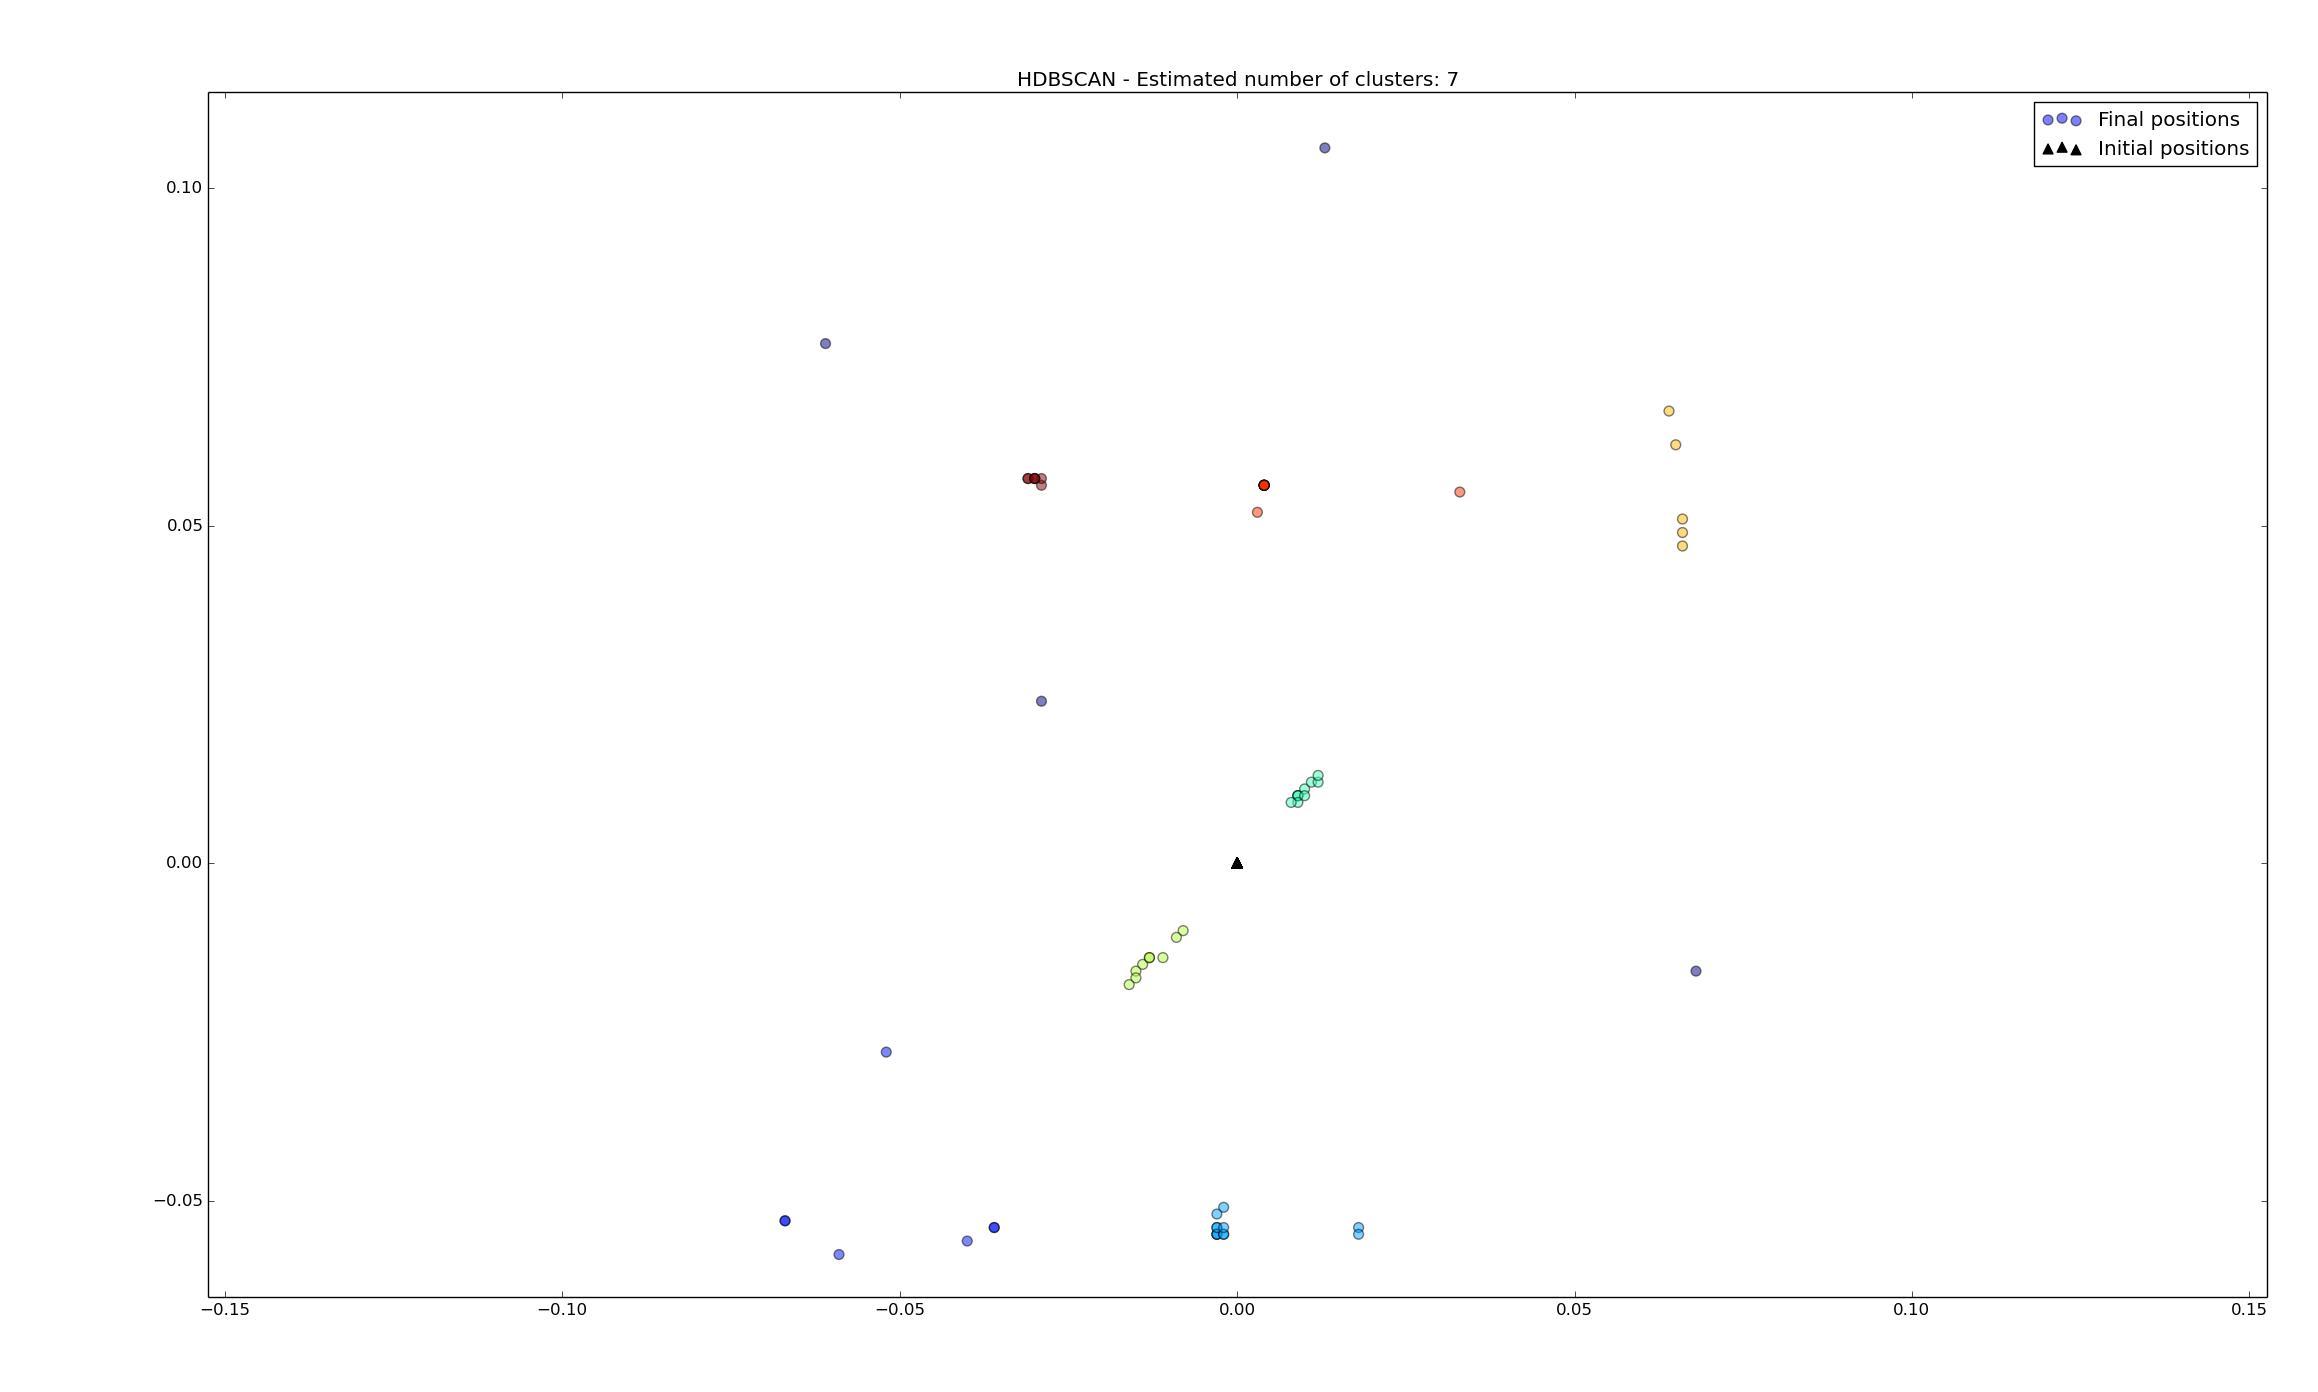
\includegraphics[width=\textwidth]{figures/ds4_non_normalized}
% 	\caption{}
% 	\label{fig:non_norm}
% \end{figure}
%
% \begin{figure}
% 	\centering
% 	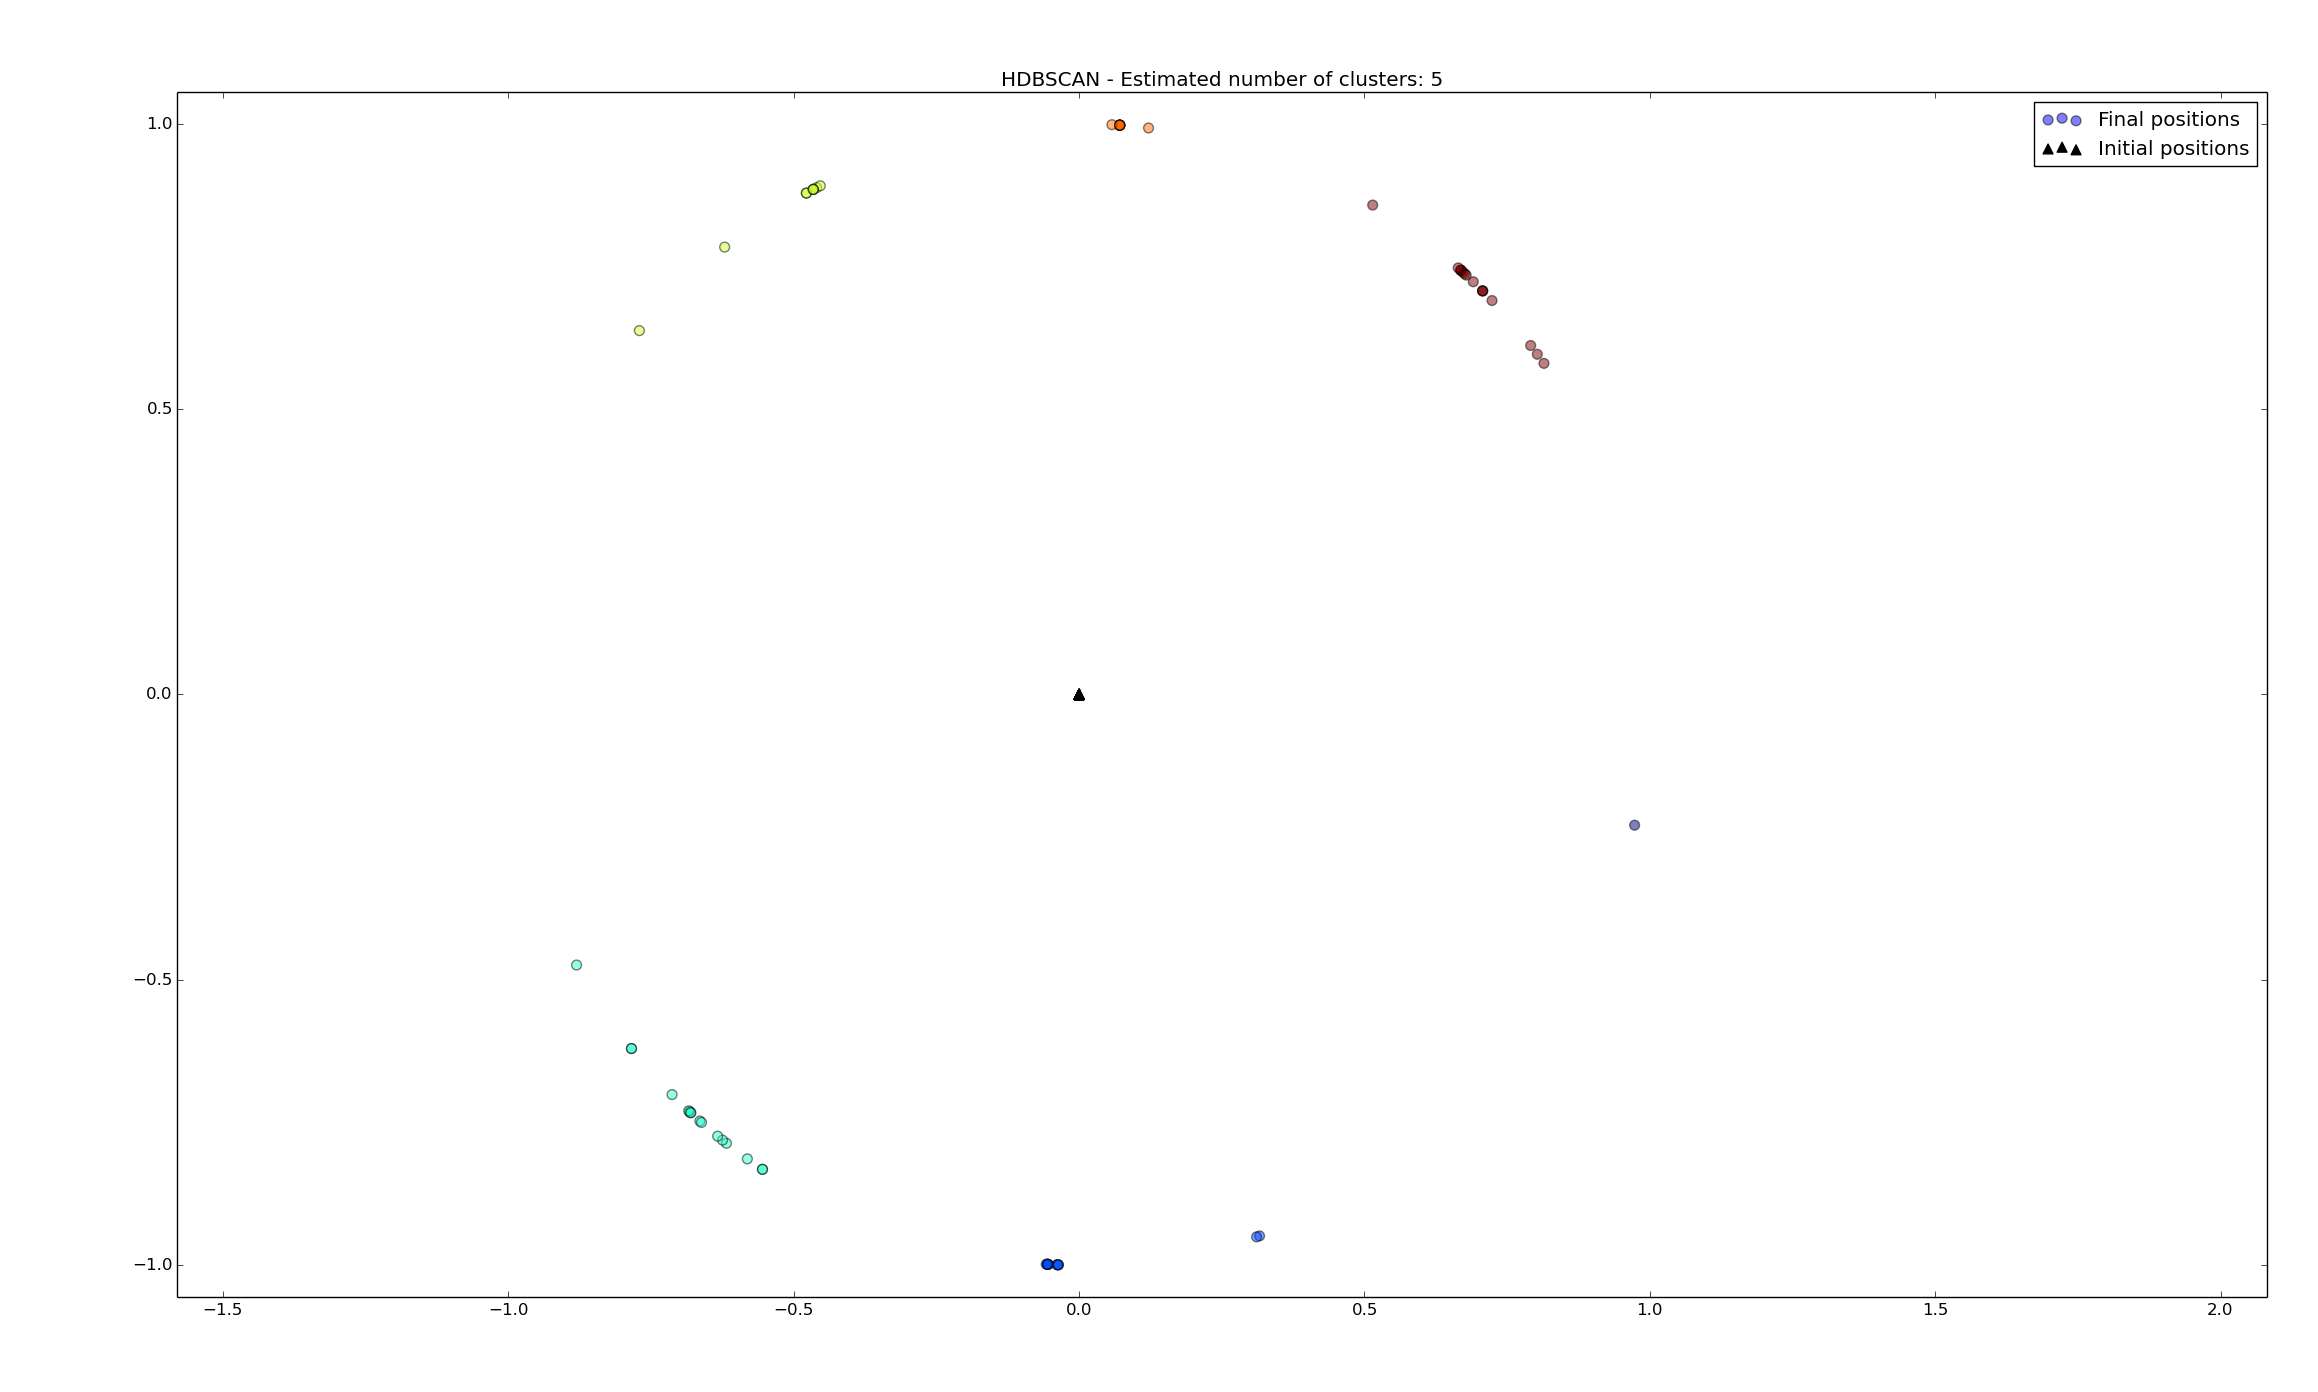
\includegraphics[width=\textwidth]{figures/ds4_normalized}
% 	\caption{}
% 	\label{fig:norm}
% \end{figure}

% \begin{figure}
% 	\centering
% 	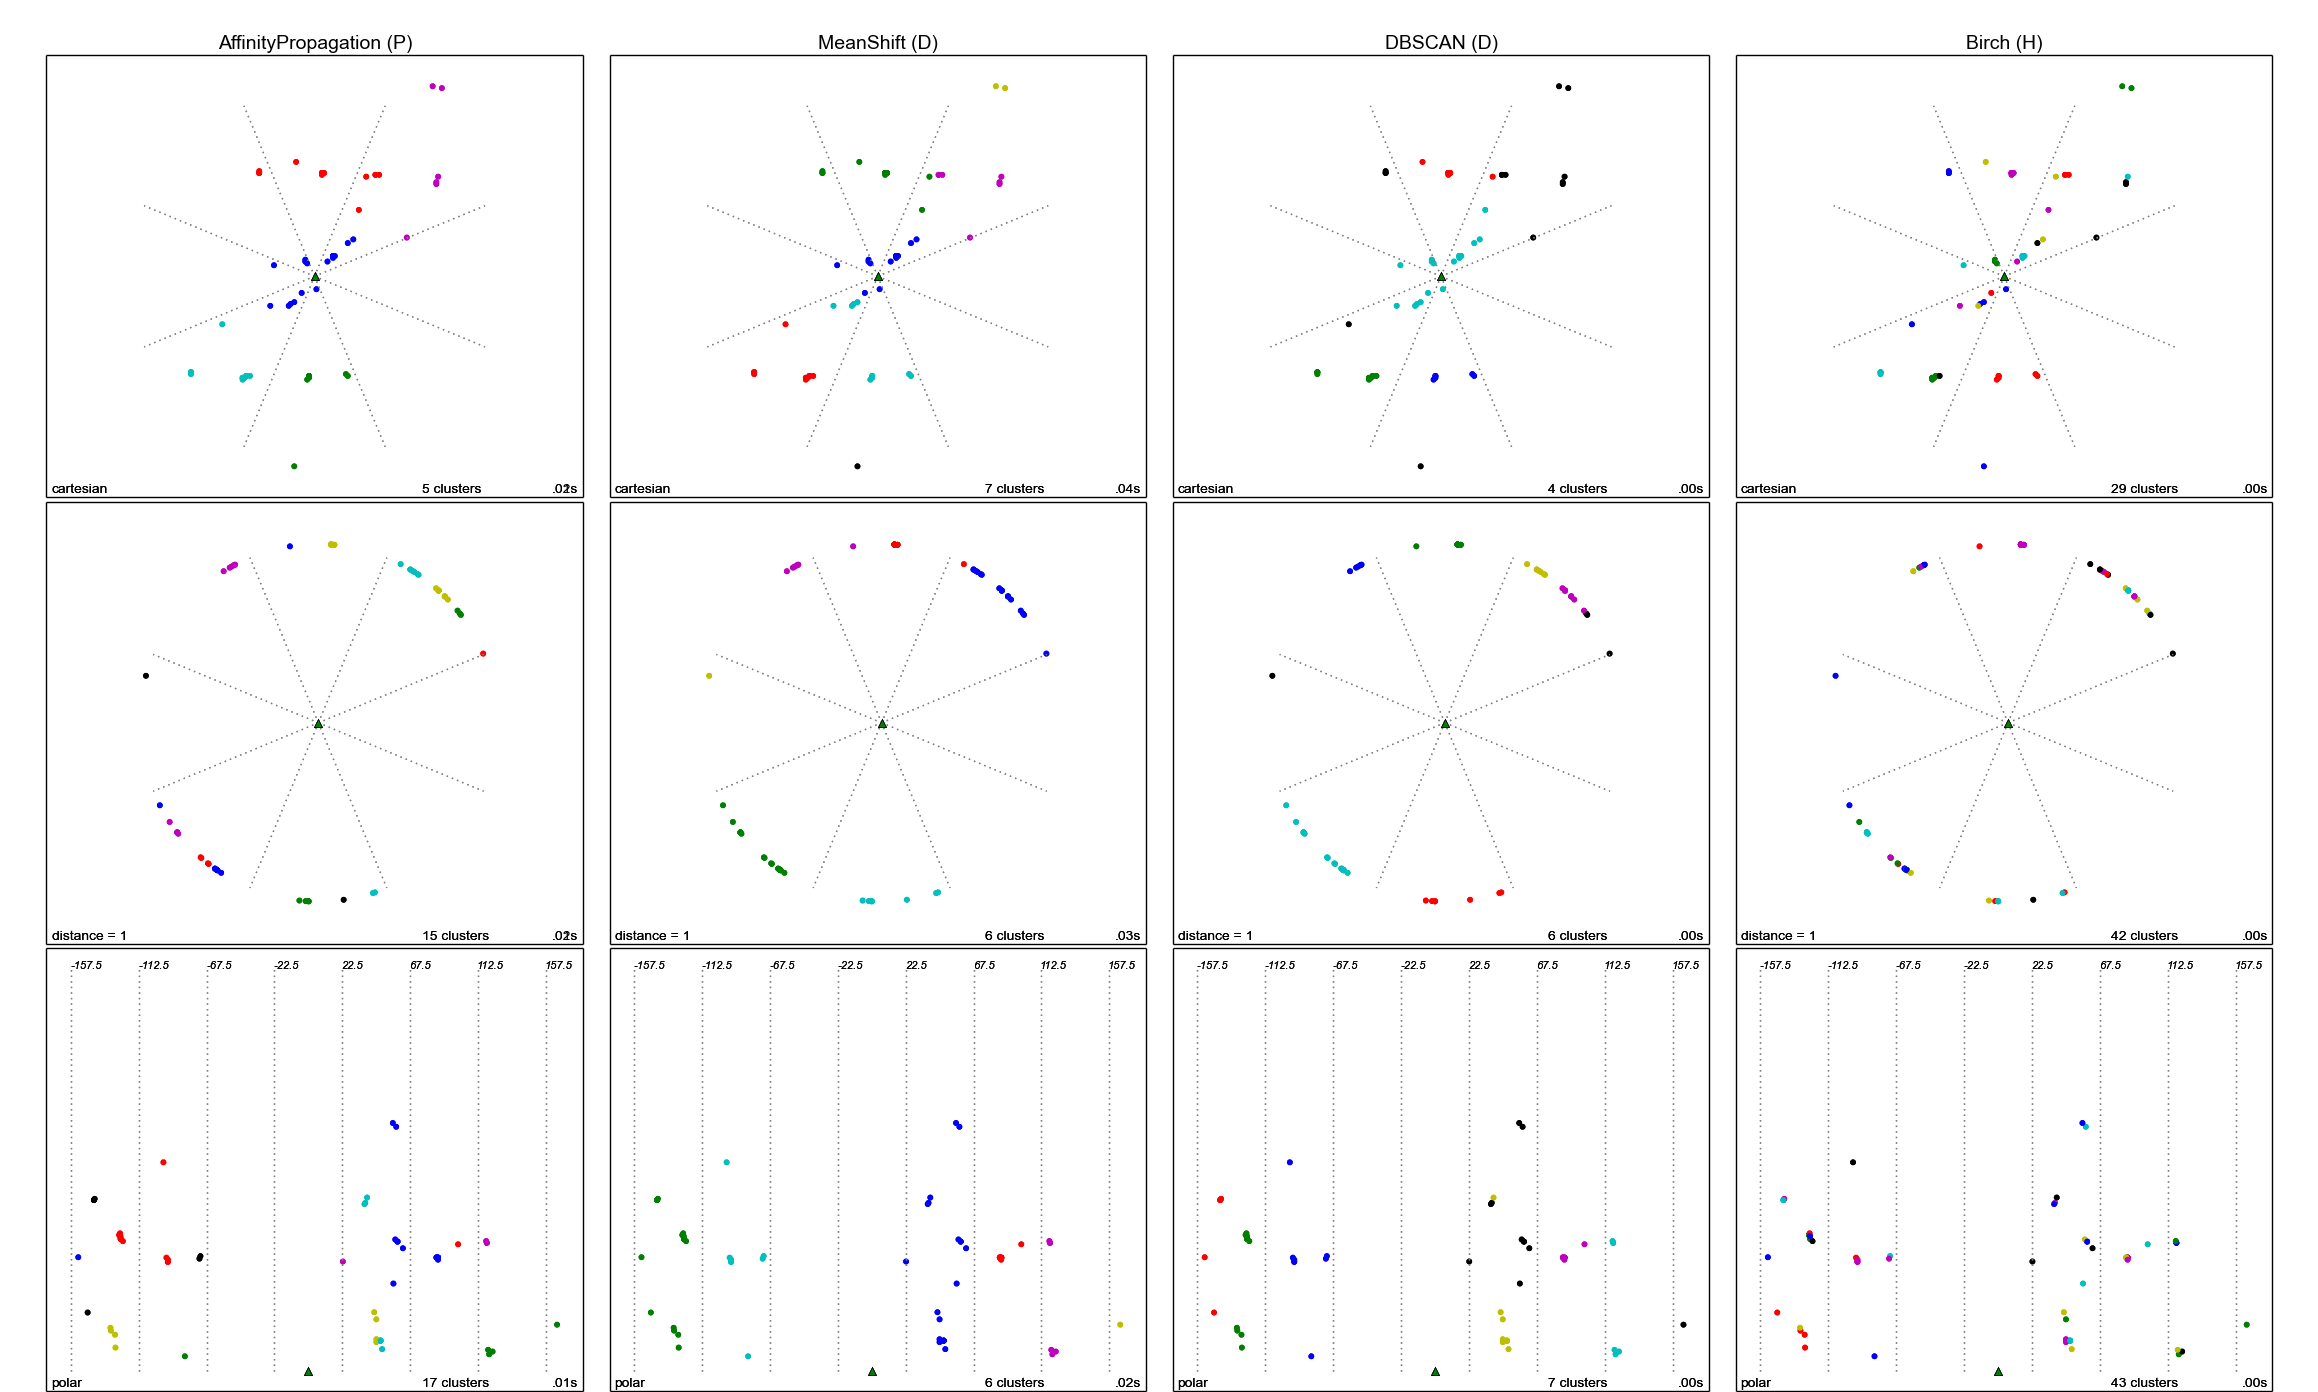
\includegraphics[width=\textwidth]{figures/comparison}
% 	\caption{Comparison between clustering algorithms. Raw data are on the first row. Below are coordinates projected in polar coordinates.}
% 	\label{fig:comparison}
% \end{figure}



% In extension of that normalisation, another solution was to convert coordinates from cartesian referential to polar referential. We found (give results...) that the clustering algorithms performed better with polar coordinates than with cartesian coordinates. Indeed, angular apertures are much more clearly distinguished. This is specially the case when values are separated with several close to the origin and others far from it.


\subsubsection{Implémentation}
Pour implémenter notre algorithme, nous avons utilisé le framework C{}\verb!++! open source Sferes \cite{Mouret2010} développé au sein de l'équipe AMAC et dédié à l'optimisation évolutionniste. Ce framework a pour avantages d'être léger, multi-coeur et facilement extensible. Sa rapidité est comparable à celle de code dédiés. De nombreux algorithmes de l'état de l'art sont inclus (par exemple : CMA-ES ou NSGA-II). La mise en place est rapide dans la mesure où il ne reste qu'à rédiger le code de la fonction fitness pour obtenir un algorithme évolutionnaire complet.



Un très grand nombre d'algorithmes de clustering existent et ont été trouvés dans l'étape précédente. Sept d'entre eux ont été sélectionnés (principalement des algorithms de partitionnemente et densité). L'enjeu conistait à trouver le meilleur algorithme et paramètres associés pour un jeu de données. Nous avions également besoin d'une méthode pour valider les paramètres trouvés. Cet algorithme est utilisé par la fonction fitness au sein de l'algorithme évolutionnaire. La méthode proposée consiste en un algorithme itératif au sein duquel un algorithme de clustering est réglé afin de satisfaire à 3 objectifs : \circled{1} le nombre de mouvements pour atteindre la cible, devant être minimisé pour faire en sorte que le robot soit le plus rapide possible, \circled{2} le nombre de clusters, devant être minimisé pour simplifier le calcul et \circled{3} la distance finale, à minimiser pour la précision du contrôle. Dans la mesure où plusieurs objectifs sont à minimiser, nous avons sélectionné l'algorithme évolutif NSGA-II\cite{Deb:2002:FEM:2221359.2221582} pour remplir cette tâche.

\begin{algorithm}
\caption{Evaluation algorithm for fitness function}\label{euclid}
  \begin{algorithmic}[1]
    \State $E$ = \{C\textsubscript{e1}, \dots, C\textsubscript{en}\} \Comment{Set of clusters containing effects}
    \State $F$ = \{f\textsubscript{1}, \dots, f\textsubscript{n}\} \Comment{Set of final points}
    \State $I$ = (0;0) \Comment{Initial point}
    \State $t$ = 0 \Comment{Number of tries}
    \State Compute the set of effects $E$ from genotype
      \ForAll{final point $f\textsubscript{i}$ in $F$}
        \For{$j=1$ to \textit{nb\_repeat} }
          \While{$dist(I,\:f\textsubscript{i}) > \varepsilon$ \textbf{and} $t<t_{max}$}
            \State $M = \{ m\textsubscript{i}\:|\:m\textsubscript{i} = rand(C\textsubscript{ei})\:\forall\:C\textsubscript{ei}\:\in E\}$
            \State $m = \operatornamewithlimits{argmin}\limits_{m_i \in M}(dist(I+m\textsubscript{i},\:f\textsubscript{i}))$
            \State Apply movement $m$ to $I$
            \State $t = t + 1$
          \EndWhile
        \EndFor
      \EndFor
      \State return (\textoverline{nb movements}, nb clusters, \textoverline{final distance})
  \end{algorithmic}
\end{algorithm}

La validation expérimentale de notre méthode a été effectuée en utilisant l'algorithme \textit{Mean Shift}, qui a révélé empiriquement la génération de clusters plus divers que \textit{X-means} lorsque ses paramètres ont été changés. Le génotype est constitué par la valeur d'un seul paramètre décimal associé à cet algorithme. La population initiale est constituée de 32 individus, évalués durant 25 générations. Les taux de croisement et de mutation pour NSGA-II sont respectivement de 0.8 et 0.1. Nous avons utilisé un jeu de données généré par un babillage orienté-objet simulé (voir ). Un point final a été aléatoirement généré au début de l'expérience. La fitness a été évaluée 30 fois pour chaque individu, les valeurs moyennes des objectifs étant ensuite reportées.

Les résultats ont été comparés avec une discrétization obenue par une recherche de type \textit{Grid Search} dans l'espace de paramètres. Le résultat obtenu est une succession de graphiques représentant les différents clusters obtenus avec les différentes valeurs de paramètres. Des exemples de clusters obtenus pour différentes valeurs du paramètre \textit{quantile} de \textit{Mean Shift} sont listés dans la figure \ref{fig:validation}.

\begin{figure}[ht]
  \begin{center}
  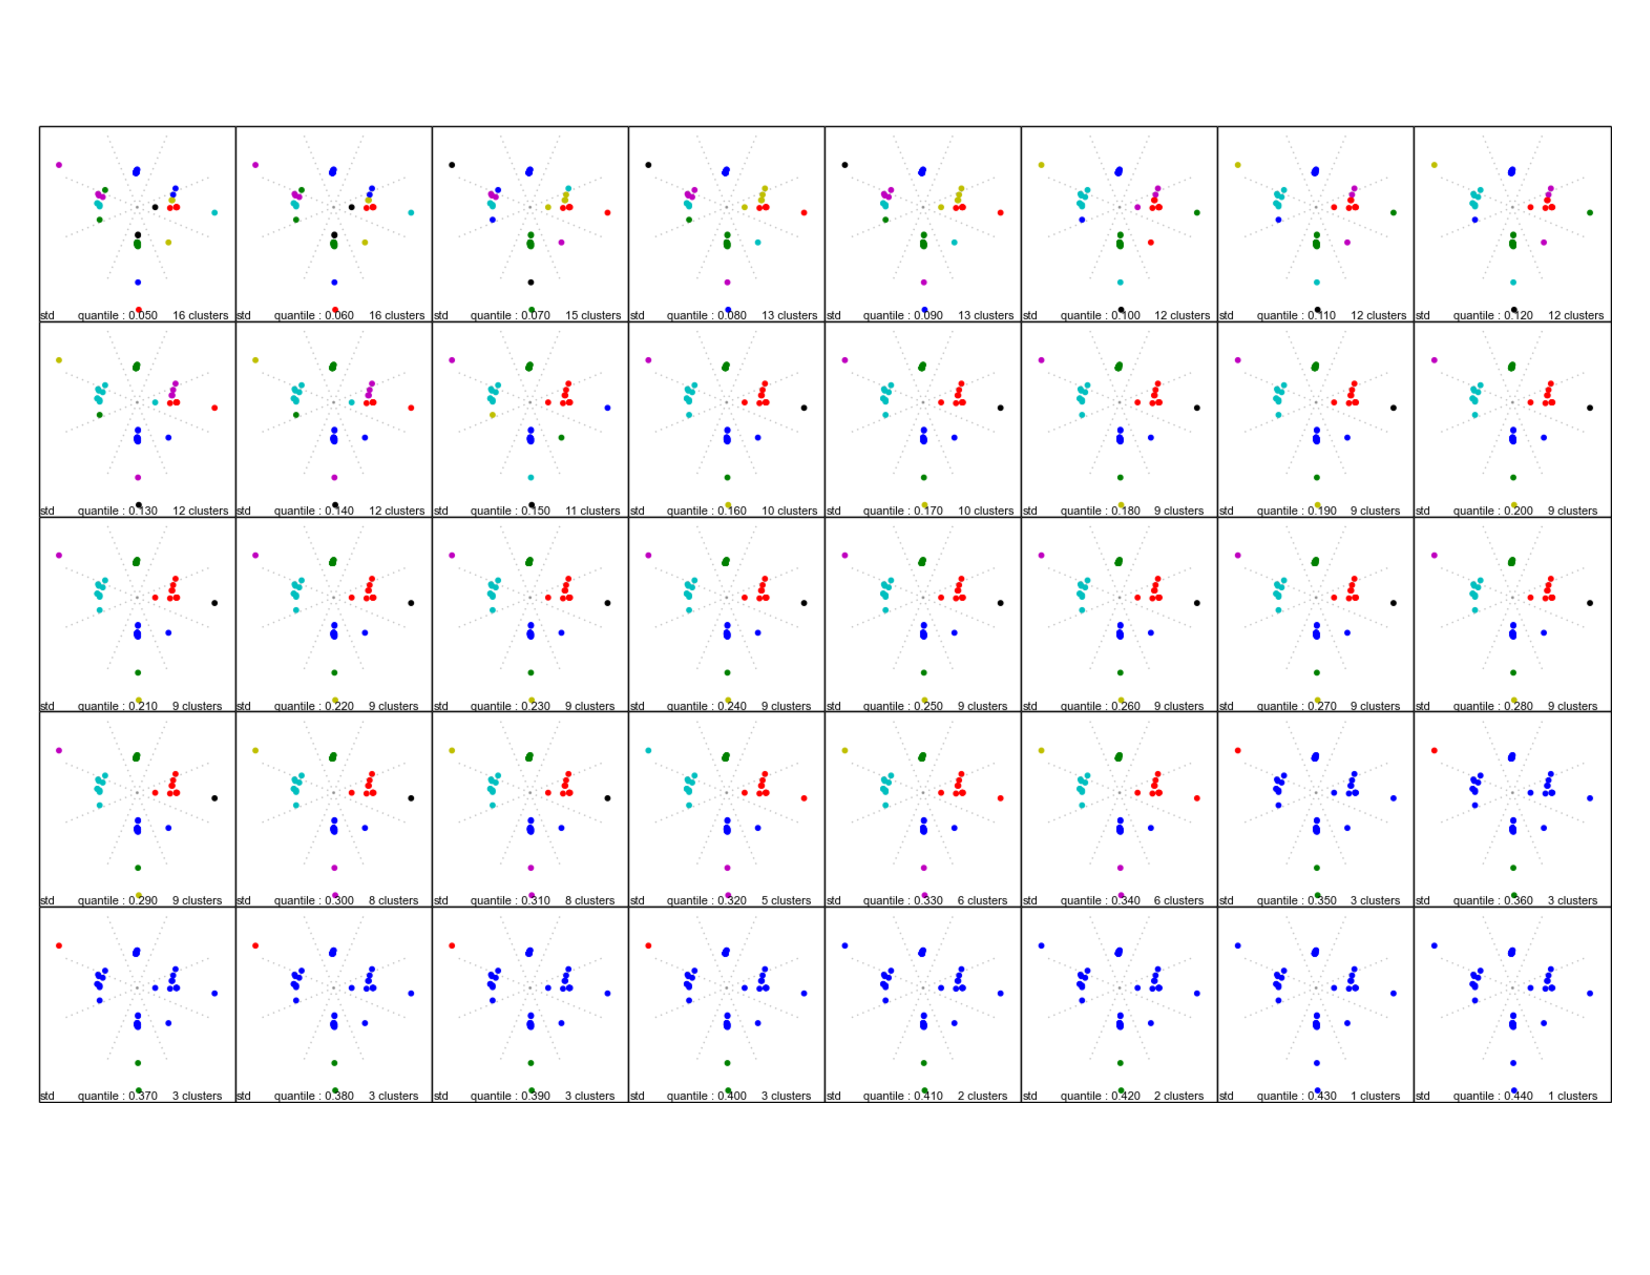
\includegraphics[width=\textwidth]{figures/DS2_MS.pdf}
    \caption{Clusters en fonction de l'évolution du paramètre \textit{quantile} de l'algorithme \textit{Mean Shift}. Les valeurs sont comprises dans l'intervalle [0.050;0.44].}
  \label{fig:validation}
  \end{center}
\end{figure}

NSGA-II étant un algorithme multi-objectif, plusieurs meilleures solutions peuvent être trouvées, correspondants aux individus dominants le front de Pareto. La figure \ref{fig:pareto_front} montre la valeur du paramètre (de l'algorithme de clustering) correspondant aux individus dominants. Différentes valeurs peuvent être relevées, par exemple 0.05, 0.12 ou 0.31.

\`A partir de cet ensemble de meilleures valeurs de paramètres, nous avons généré (Figure \ref{fig:results}) deux séries de graphiques. Les deux ensembles de clusters optimisent différents objectifs : vitesse et précision pour celui de gauche contre coût computationnel pour celui de droite. La colonne de gauche contient davantage de clusters et permet un contrôle rapide et précis. \`A l'inverse, l'autre solution repose sur un nombre moins important de clusters.

\begin{figure}[!tbp]
  \centering
  \begin{minipage}[b]{0.4\textwidth}
    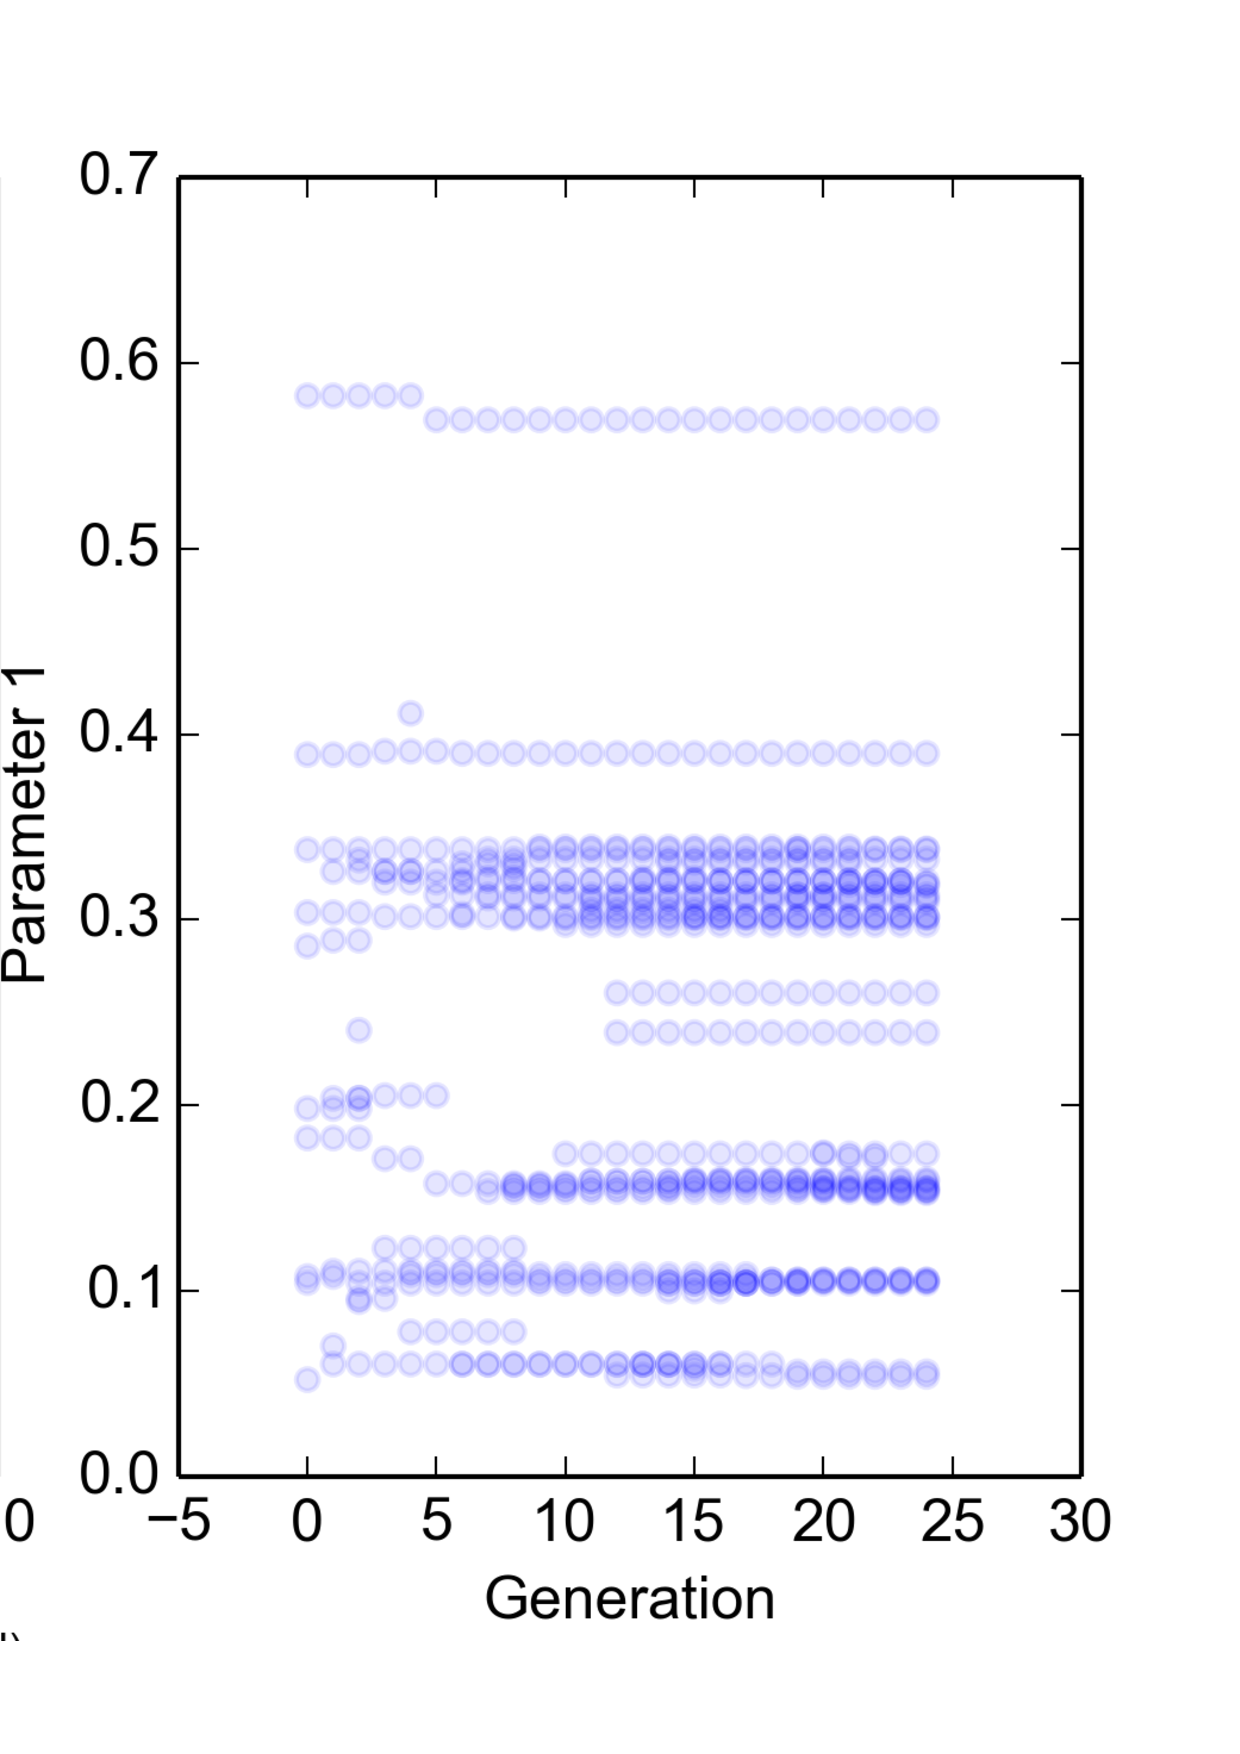
\includegraphics[width=\textwidth]{figures/Pareto_front.pdf}
    \caption{Valeur du paramètre de l'algorithme de clustering Mean Shift correspondant aux individus dominants le front de Pareto. Plusieurs valeurs se détachent, par exemple $0.05$, $0.11$ ou $0.3$.}
    \label{fig:pareto_front}
  \end{minipage}
  \hfill
  \begin{minipage}[b]{0.5\textwidth}
    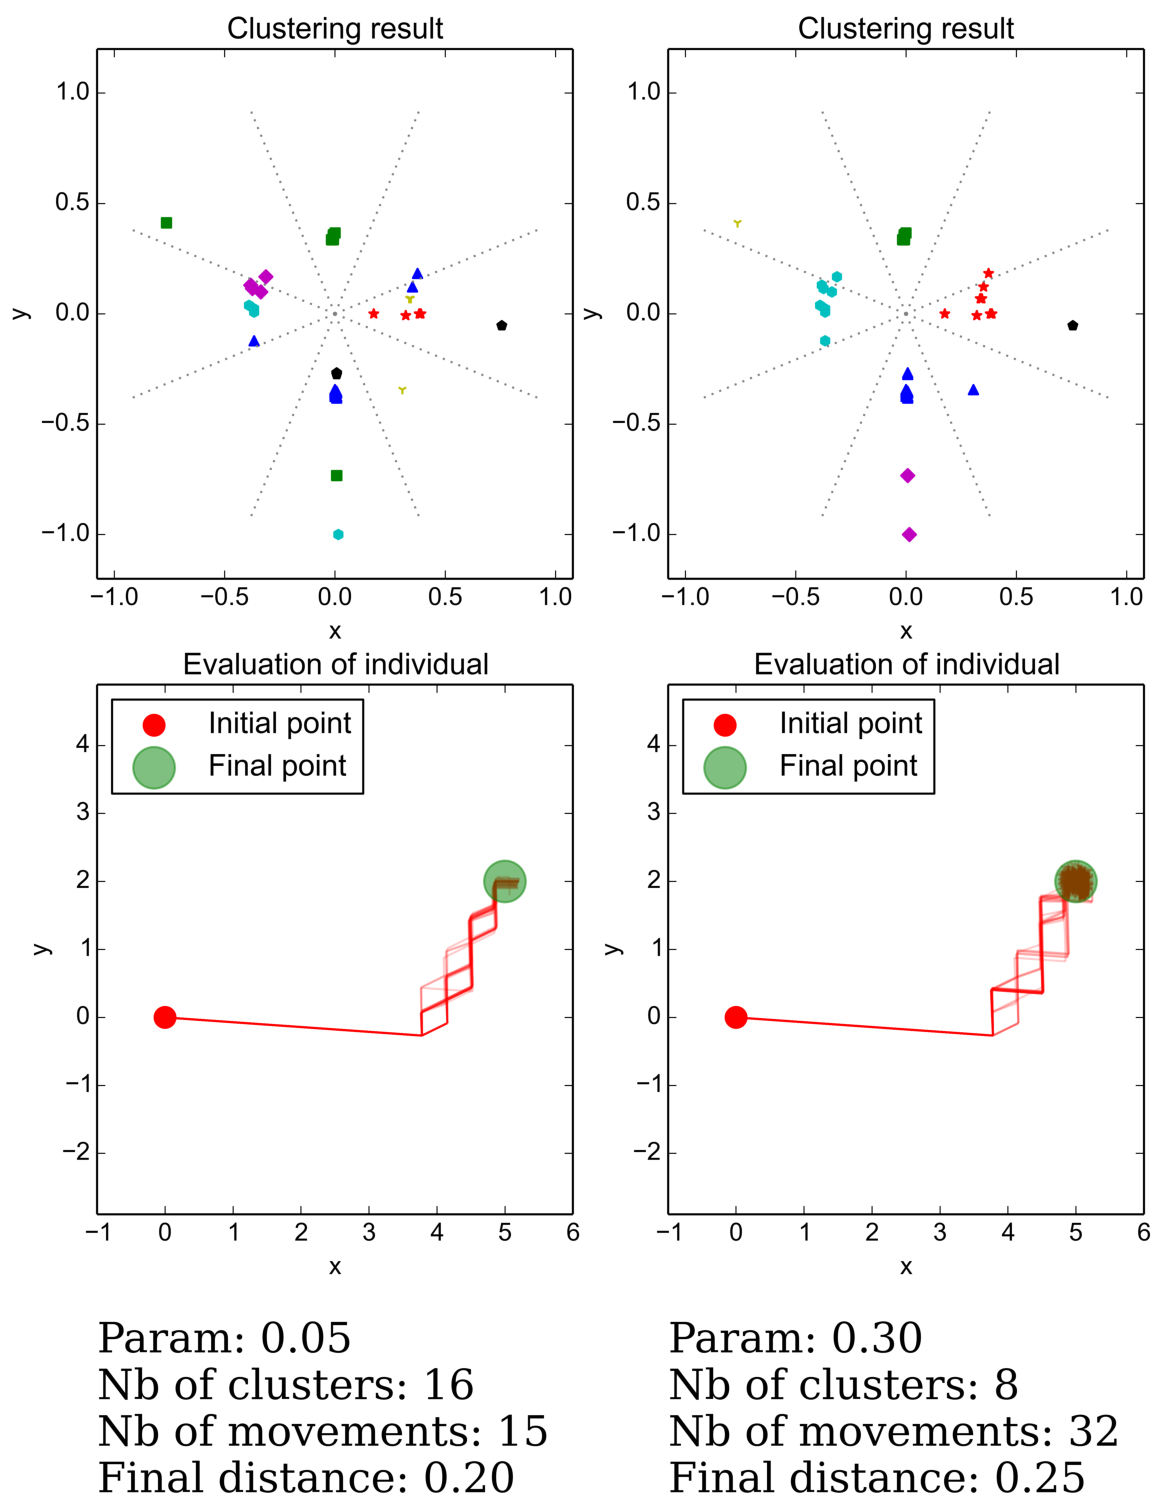
\includegraphics[width=\textwidth]{figures/Benchmark_3.pdf}
    \caption{Les deux colonnes montrent différents résultats de clustering et de trajectoires d'évaluations basés sur les valeurs de paramètres appartenant aux individus dominants le front de Pareto.}
    \label{fig:results}
  \end{minipage}
\end{figure}


Clusterisation based on Ugur's paper: 40 features. Compare Ugur's work with us.\\

Cette première partie de notre stage a fait l'objet d'une soumission d'un abstract au workshop \textit{Developmental learning and representation building in human-robots and ambient intelligence systems} de la conférence ECAL2017\footnote{https://project.inria.fr/ecal2017/} qui se tient à Lyon en septembre 2017.






\subsection{Expérience de validation}
La seconde partie de notre stage a consisté à mener une expérience pour valider l'algorithme de clusterisation d'effets défini dans la première partie de ce mémoire. Dans un premier temps, l'expérimentation a eu lieu en simulation. Une fois cette simulation validée, le robot réel a été utilisé. Cette expérience peut être divisée en 3 étapes : \circled{1} génération du babbling sensorimoteur et enregistrement des effets pour les différents objets, \circled{2} réalisation de la clusterization des effets et \circled{3} test de l'apprentissage.  La figure \ref{fig:setup} représente la mise en place initiale de l'expérimentation.

\subsubsection{Babillage}
Durant la première étape de cette expérimentation, un objet (par exemple, un cube) est placé sur la table à une position initiale. Un babillage sur l'objet est réalisé afin d'obtenir ses jeux de données contenant les différents effets découverts à traiter. Ce babillage est effectué à l'aide de l'algorithme \textit{NovEB} décrit par Maestre et al.\cite{Maestre2015}. Cet algorithme utilise l'algorithme évolutionnaire \textit{Novelty Search}\cite{5949955} pour générer des trajectoires permettant d'atteindre un objet dans le cadre d'un babillage. Pour cela, le calcul des trajectoires est effectué dans un premier temps \textit{via} sélection/mutation. Puis, pour chaque trajectoire, l'on regarde si elle intersecte avec le cube. Si c'est le cas, cette trajectoire est gardée et jouée par le robot en simulation. La figure \ref{fig:ns_traj} montre un exemple de trajectoire touchant l'objet considéré.

\begin{figure}[!tbp]
  \centering
  \begin{minipage}[b]{0.4\textwidth}
    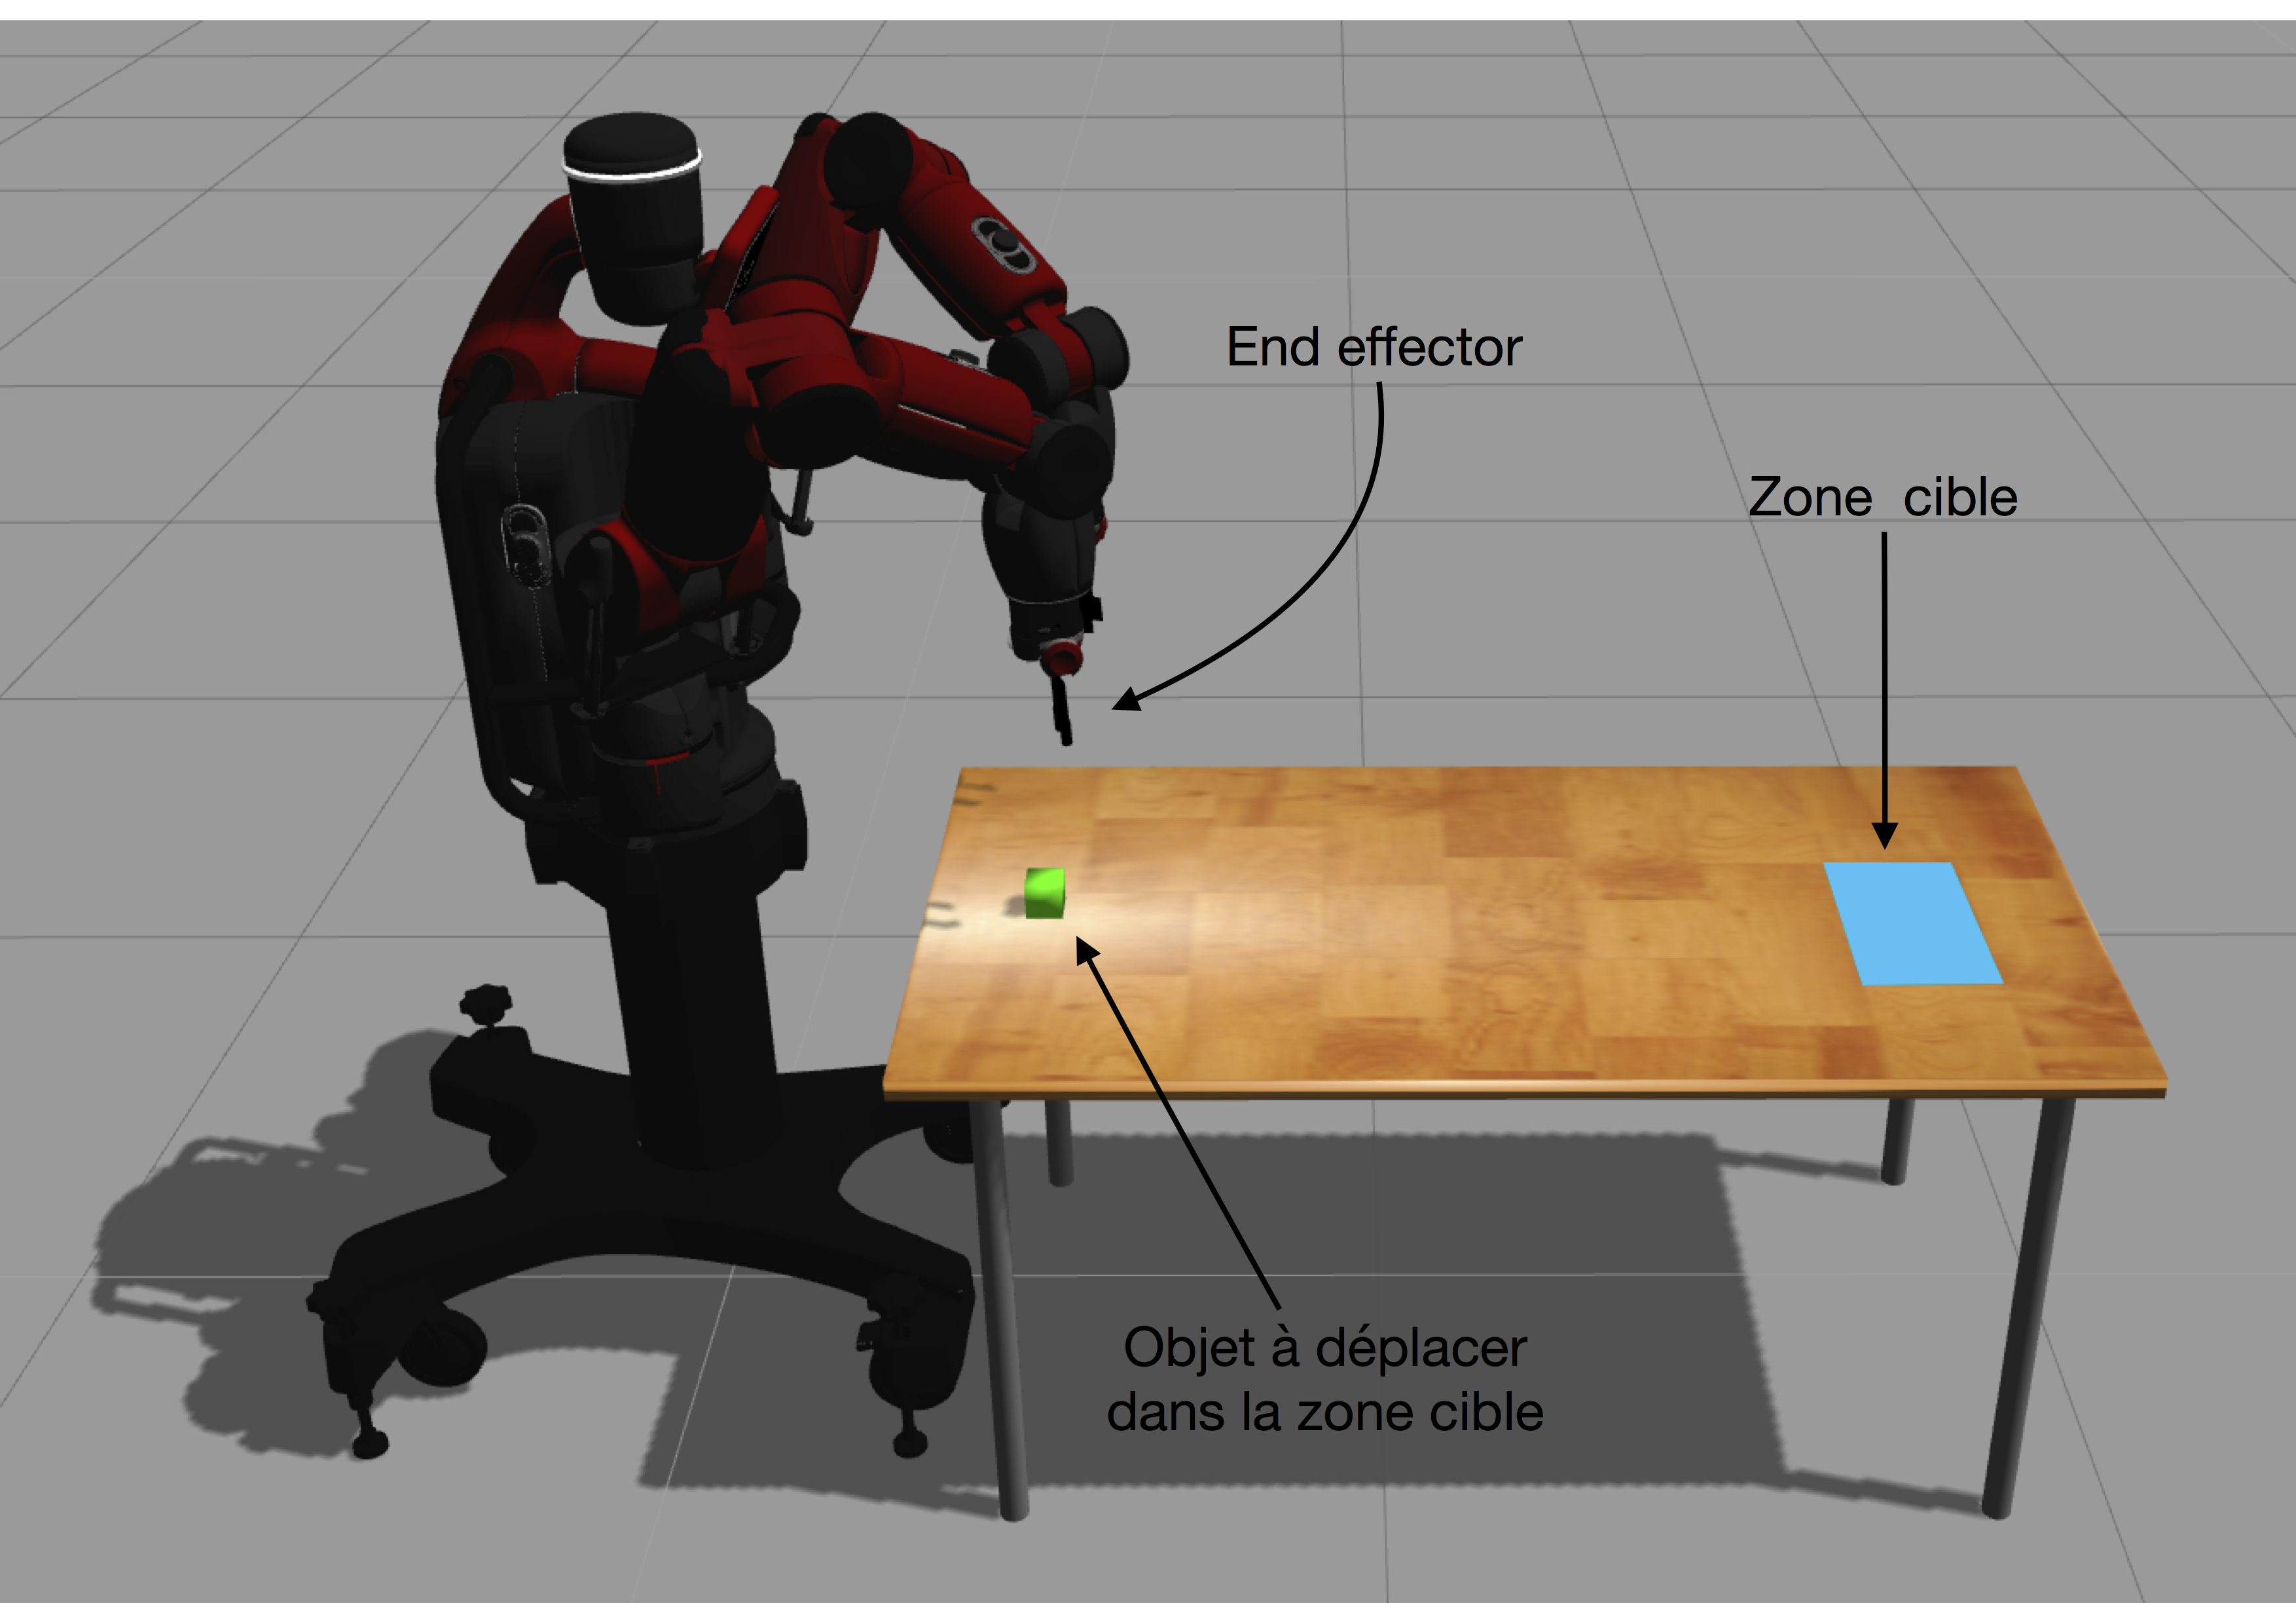
\includegraphics[width=\textwidth]{figures/Experiment_setup_annoted_FR.png}
    \caption{L'objectif du robot est d'apprendre à pousser différents objets (par exemple, le cube vert) depuis sa position initiale jusqu'à la zone cible en bleu. Une première étape de babillage permet de découvrir les effets qui sont clusterisés à l'aide de l'algorithme de clusterisation. Enfin, dans une troisième étape, le robot tente d'atteindre la zone cible.}
    \label{fig:setup}
  \end{minipage}
  \hfill
  \begin{minipage}[b]{0.4\textwidth}
    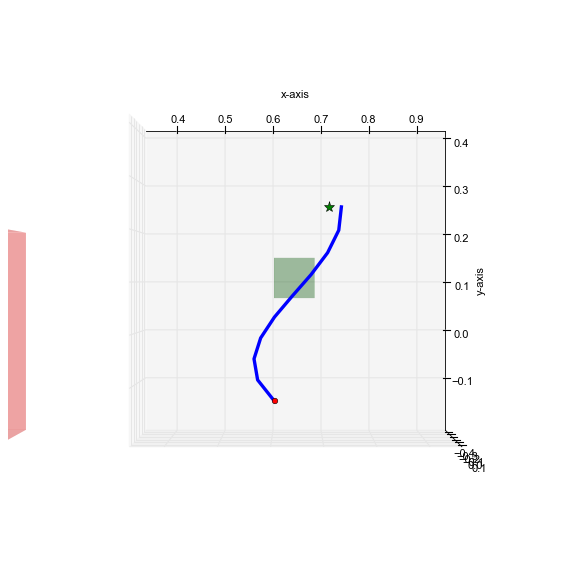
\includegraphics[width=\textwidth]{figures/ns_trajectory.png}
    \caption{Génération de trajectoire avec NovEB. Le rectangle rouge représente l'emplacement du robot. Le point rouge correspond à la position initiale de l'effecteur du robot. Le tracé en bleu correspond à la trajectoire de cet effecteur vers l'objet. L'étoile verte indique la position de l'objet à la fin de l'exécution de la trajectoire de l'effecteur.}
    \label{fig:ns_traj}
  \end{minipage}
\end{figure}


% Ces objets ont différentes propriétés : certains peuvent être poussés à partir de n'importe quelle face et générer un comportement identique (boîte), tandis que d'autres nécessiteront d'être poussés depuis une face particulière (cylindre et cône) afin de garder une trajectoire cohérente. Le babillage réalisé par le robot sur ces différents objets permet de produire des jeux de données d'effets.
\subsubsection{Clusterisation d'effets}
La seconde étape implique l'algorithme que nous avons présenté ci-dessus et vise à clusteriser les effets présents dans les jeux de données. Il en résulte une variété de paramètres qui peuvent être exploités durant la troisième étape.
Les meilleurs paramètres trouvés dans l'étape précédente sont utilisés pour pousser les différents objects vers la zone cible. Dans notre expérience, une valeur du paramètre \textit{quantile} est sélectionnée (par exemple, 0.18) et utilisée pour générer le clustering utilisé par le robot.

% La première étape consiste donc en un babillage. Concrétement, la position de l'objet sur l'espace de travail est récupérée ainsi que la position de l'effecteur. Une trajectoire est ensuite générée à l'aide de la cinématique inverse et Novelty Search afin d'atteindre l'objet. Cet objet est positionné de façon aléatoire dans les intervalles [x;x] et [y;y].

\subsubsection{Poussée de l'objet}
Enfin, dans un troisième temps, le robot tente de pousser l'objet présenté devant lui vers une zone cible (dont la position est variable), en utilisant les différents effets à sa disposition, trouvés lors de l'étape précédente. Cette dernière étape soulève plusieurs problèmes qu'il a fallu résoudre. 

Tout d'abord, concernant la position de l'effecteur. Les effets générés lors du babillage sont effectués à partir de différentes faces de l'objet. Ainsi, lorsque le robot tente de pousser l'objet vers la zone cible, en fonction de la position de cette zone à atteindre, les effets seront différents ainsi que les faces/points de contacts d'où initier les effets. \`A chaque effet est associé un point de contact dans le repère de l'objet. Cela nous a amené à récupérer les coordonnées du point de contact pour savoir d'où initier l'effet. Ces coordonnées sont exprimées dans le repère lié à l'objet et sont corrélées à l'effet enregistré. La figure \ref{fig:contact_position} présente ce cas particulier.



\begin{figure}[ht]
  \begin{center}
  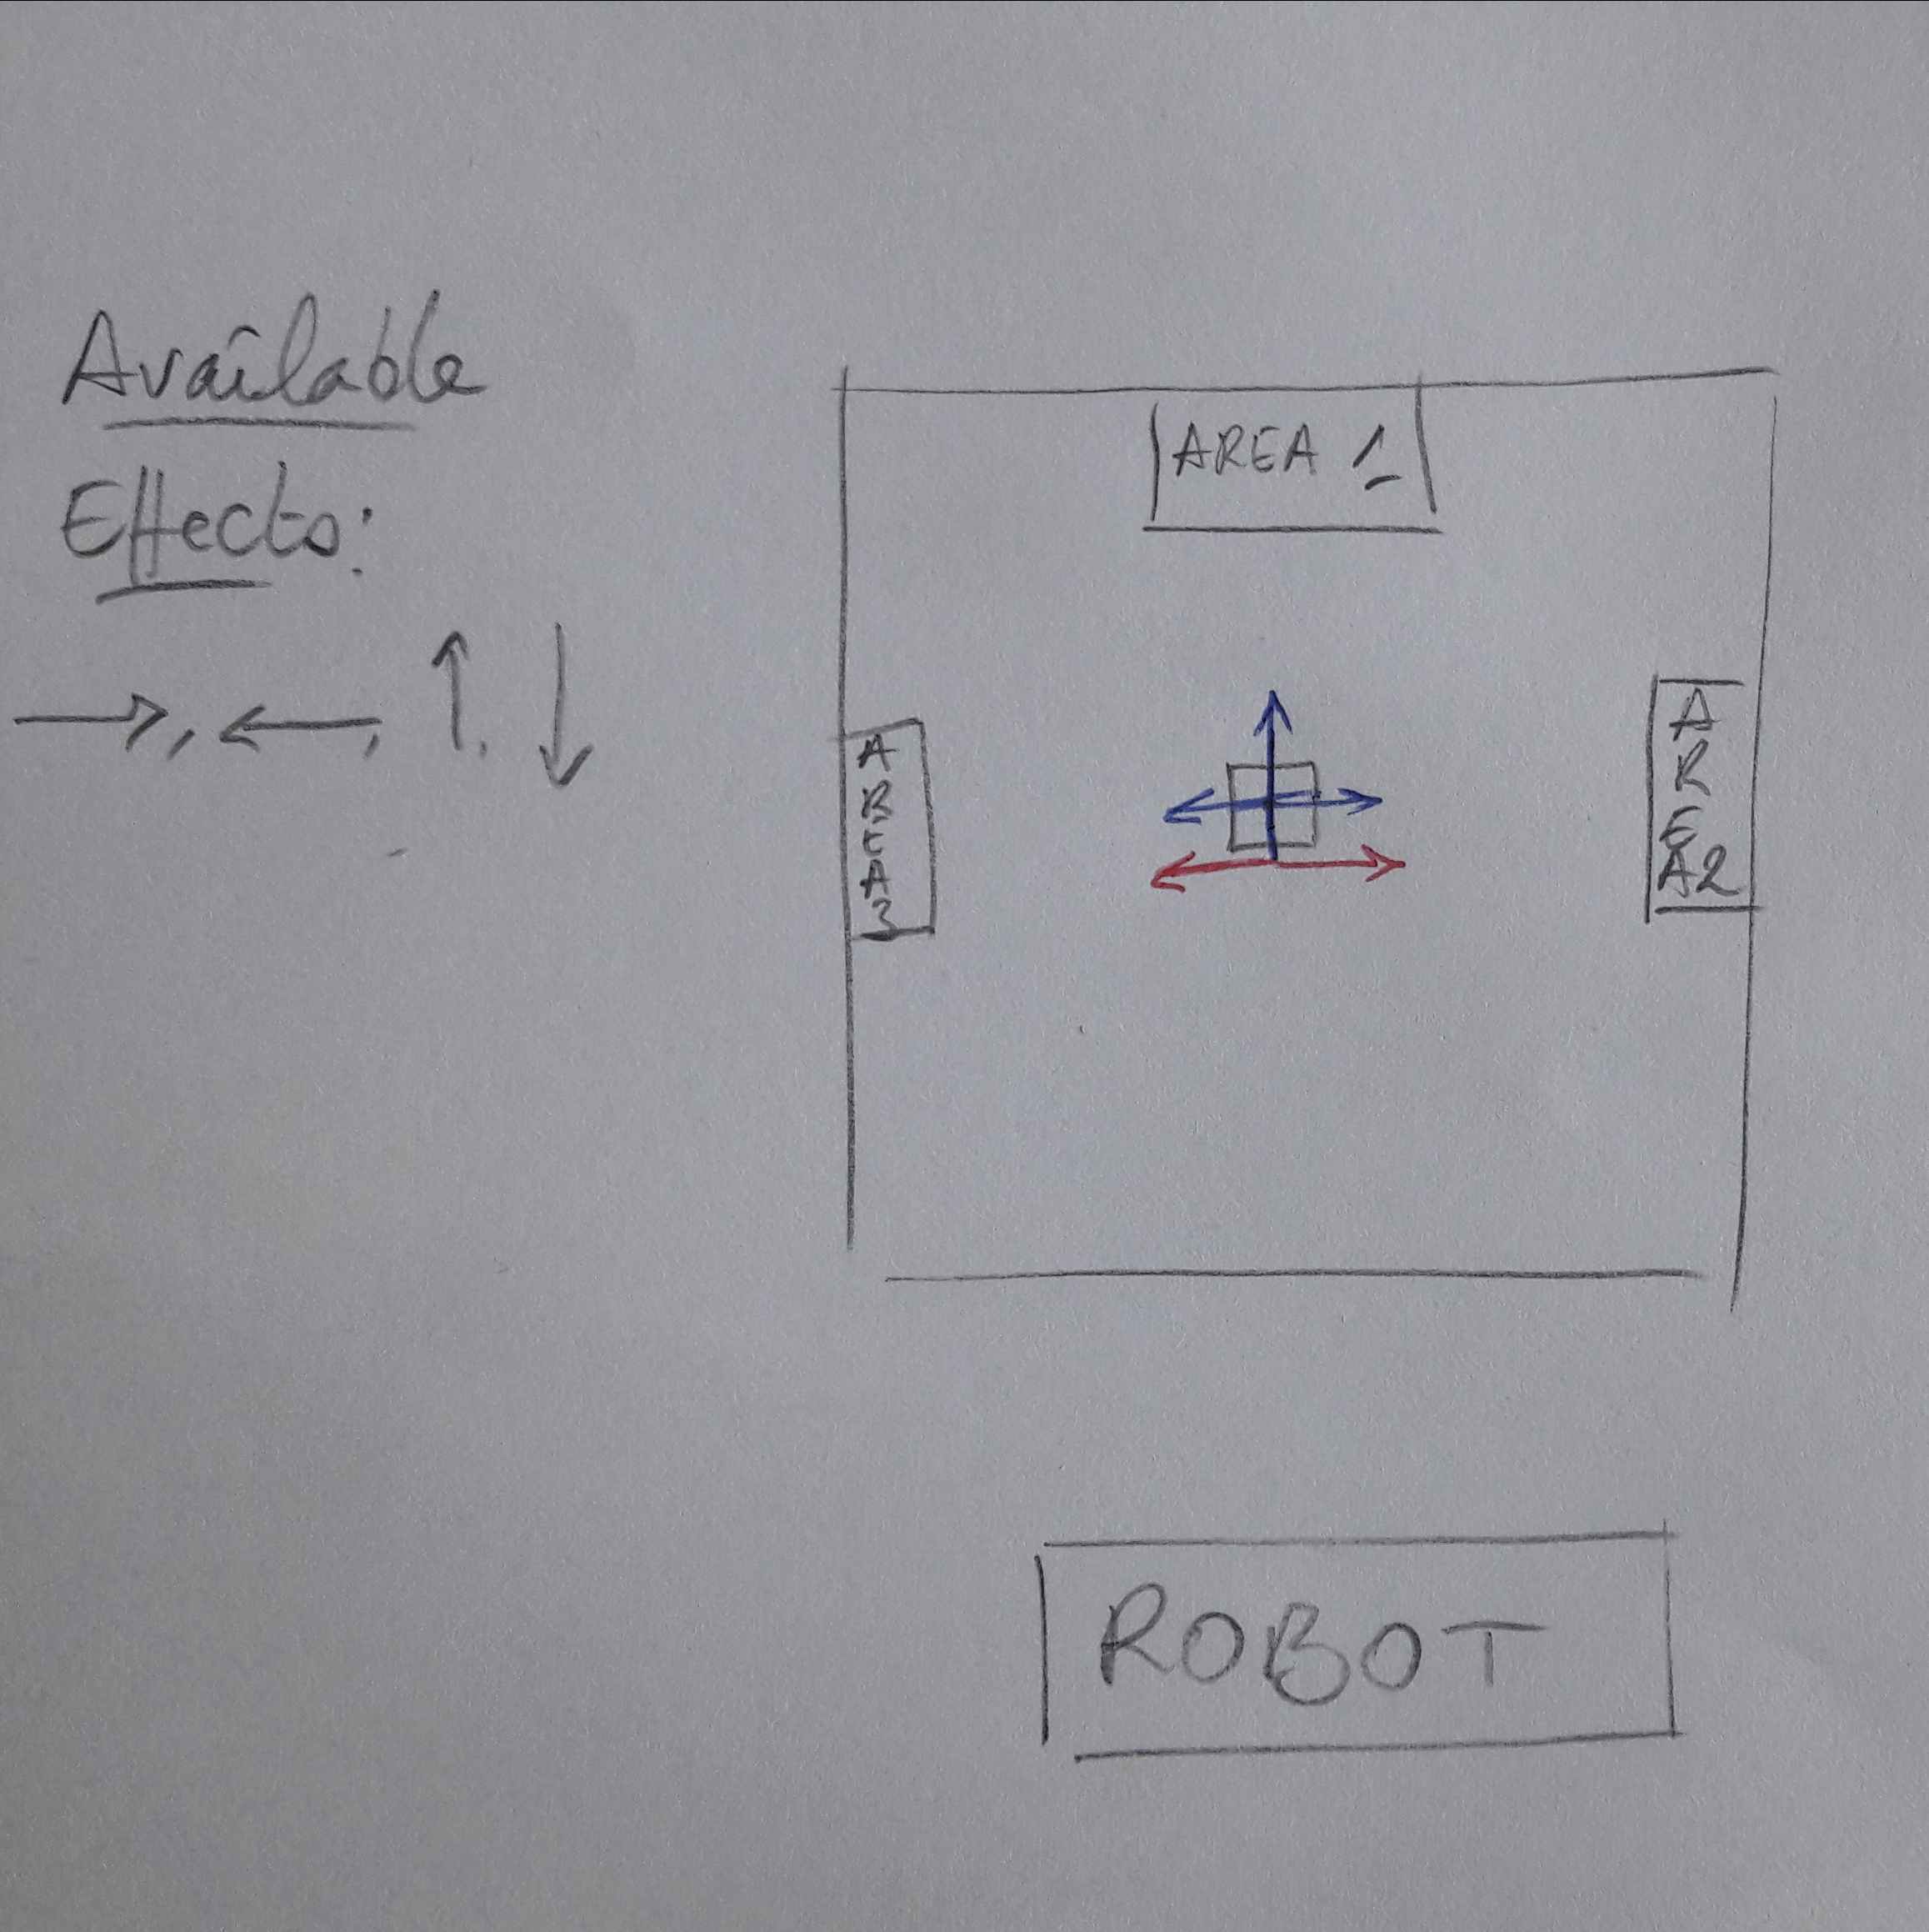
\includegraphics[width=0.4\textwidth]{figures/contact_position.jpg}
    \caption{Les coordonnées du point de contact de l'effecteur sur l'objet permettent de positionner correctement l'effecteur lors de la phase de poussée. Cette indication est d'autant plus importante avec des objets ayant des propriétés particulières (cylindre, cône).}
  \label{fig:contact_position}
  \end{center}
\end{figure}

Le second problème a trait avec la tâche elle-même : l'objectif visé n'est pas de pousser simplement un objet jusqu'à une zone finale, mais d'effectuer une geste avec une vélocité élevée afin de pousser fortement l'objet jusqu'à la zone inacessible pour le bras du robot. Utilisation de Quality Diversity pour effectuer le babillage concernant la vélocité.

\subsubsection{Résultats}
Les premiers résultats provenant de cette expérimentation montrent que le robot est tout à fait capable de pousser un objet vers une zone particulière en se basant sur la discrétisation d'effets obtenue par babillage sensorimoteur. Une vidéo est disponible en ligne : youtu.be/test



% During the first step, several different objects are placed on the table, one after another. Those objects have different properties: a box, a cylinder which and a cone. Some can be pushed from any face and will have the same behavior, whereas the other ones need to be pushed from a particular face to move significantly. The babbling with the different objects would result in a dataset of effects.
% The second step implies the algorithm we presented above and tries to clusterize the effects in the dataset. As result, a variety of parameter can be exploited during the third stage.
% The best parameters found in the previous stage are used for pushing the different object into the goal area.

\section{Discussion}
% \epigraph{A computer would deserve to be called intelligent if it could deceive a human into believing that it was human.}{\textit{Alan Turing}}







\section{Travaux futurs et perspectives}

Plusieurs axes d'améliorations peuvent être proposés. Durant ce stage, nous avons testé l'algorithme présenté ci-dessus avec un seul algorithme de clustering, \textit{Mean Shift}. Le premier axe d'amélioration consisterait à tester davantage d'algorithmes de clustering, tels qu'\textit{Affinity Propagation}, \textit{Birch} ou \textit{DBSCAN}. Un second axe d'amélioration pourrait être de tester l'algorithme avec des tâches plus complexes.

Concernant l'expérience utilisant la clusterisation d'effets, il pourrait être pertinent de la réaliser en utilisant d'autres objets ayant différentes propriétés : un cylindre et un cône. Le cylindre a pour particularité de rouler sur une grande distance rectiligne lorsqu'il est poussé depuis sa face courbe alors que ce mouvement est plus réduit lorsqu'il est poussé depuis l'une de ses bases. A l'inverse, un cône décrit une courbe s'il est poussé depuis sa face courbe et nécessite d'être poussé depuis sa base pour parcourir une grande distance rectiligne. Un babillage avec ces deux objets pourrait permettre au robot d'apprendre à repositionner les objets afin d'exposer leur face appropriée aux différentes actions (face courbe pour le cylindre et base pour le cône).

L'algorithme décrit dans ce mémoire a été utilisé pour une expérience réalisée en collaboration avec UDC et ISIR en vue du de la réunion d'évaluation du projet qui se tient mi-septembre. Cette expérience consiste à faire en sorte que le robot puisse atteindre différentes zones matérialisées par des zones RFID. Utilisation du Reinforcement Learning.






\section{Conclusion}

Ce stage de fin d'études de Master 2 m'a permis de davantage découvrir le domaine de la robotique développementale et ce qu'il implique, après la brève introduction que nous avons eu durant le semestre de M2 à Lyon. Ce domaine de recherche est fascinant et très intéressant dans la mesure où les chercheurs tendent à créer des robots qui pourraient boostrap from almost no knowledge. Le lien étroit entre neurosciences et spécialement neurosciences cognitives permet d'implémenter des modèles présent chez l'être humain.

Le sujet abordé dans ce stage pointe la difficulté que représente la conception d'un robot autonome et capable d'apprendre en permanence dans son environnement.

In that paper, we have proposed an approach to allow a robot learn from its own experiments and exploit babbling data in order to identify sets of reachable effects that define actions relevant to a task-dependant context. In the future, we will extend that approach by using more clustering algorithms and parameters, and investigate its application to more complex and varied tasks.

% \section*{Annexe}

% Liste des différentes waves

% \begin{tabular}{|l|c|r|}
%   \hline
%   No & Requirements 2 & Partners \\
%   \hline
%   W1 & Babbling & UPMC \\
%   W2 & Saliency Learning & UPMC \\
%   W2 & Saliency Learning & UPMC \\
%   W3 & Object Babbling & UPMC \\
%   W4 & Object Interaction Babbling & UPMC \\
%   W5 & Object Interaction discretization & UPMC \\
%   W6a & End to End policy pre-training & QMUL \\
%   W6b & End to End policy fine tuning & QMUL \\
%   W7 & Feature learning & Armines \\
%   W8 & Feature Based Reinforcement Learning & Armines \\
%   W9 & Policy-based exploration & Armines \\
%   W10 & Contextual Policy learning & UPMC \\
%   W11 & Model learning & UDC \\
%   W12 & Value function learning & UDC \\
%   W13 & Policy modularization & QMUL \\
%   \hline
% \end{tabular}

% Liste des différentes working packages

% \begin{tabular}{|l|c|r|}
%   \hline
%   No & Requirements 2 & Partners \\
%   \hline
%   W1 & Babbling & UPMC \\
%   W2 & Saliency Learning & UPMC \\
%   W2 & Saliency Learning & UPMC \\
%   W3 & Object Babbling & UPMC \\
%   W4 & Object Interaction Babbling & UPMC \\
%   W5 & Object Interaction discretization & UPMC \\
%   W6a & End to End policy pre-training & QMUL \\
%   W6b & End to End policy fine tuning & QMUL \\
%   W7 & Feature learning & Armines \\
%   W8 & Feature Based Reinforcement Learning & Armines \\
%   W9 & Policy-based exploration & Armines \\
%   W10 & Contextual Policy learning & UPMC \\
%   W11 & Model learning & UDC \\
%   W12 & Value function learning & UDC \\
%   W13 & Policy modularization & QMUL \\
%   \hline
% \end{tabular}

% % \addcontentsline{toc}{chapter}{Annex}
%
% % \begin{tabular}{|l|c|r|}
% %   \hline
% %   colonne 1 & colonne 2 & colonne 3 \\
% %   \hline
% %   1.1 & 1.2 & 1.3 \\
% %   2.1 & 2.2 & 2.3 \\
% %   \hline
% % \end{tabular}
%
% \begin{tabular}{ |l|l|l| }
% % \hline
% % \multicolumn{3}{ |c| }{Team sheet} \\
% \hline
% Type & Name & Since \\ \hline
% \multirow{4}{*}{Partitionnement} & LB & Lucas Radebe \\
%  & DC & Michael Duburry \\
%  & DC & Dominic Matteo \\
%  & RB & Didier Domi \\ \hline
% \multirow{3}{*}{Basé sur la densité} & MC & David Batty \\
%  & MC & Eirik Bakke \\
%  & MC & Jody Morris \\ \hline
% \multirow{2}{*}{Grid based} & ST & Alan Smith \\
%  & ST & Mark Viduka \\
% \hline
% \end{tabular}

\bibliographystyle{unsrt}
\bibliography{./LEROY_M2_ISIR_2017_internship_thesis.bib}

\end{document}
